\documentclass[svgnames,unknownkeysallowed]{beamer}
\addtobeamertemplate{navigation symbols}{}{%
    \usebeamerfont{footline}%
    \usebeamercolor[fg]{footline}%
    \hspace{1em}%
    \insertframenumber/\inserttotalframenumber
}
\setbeamertemplate{section in toc}[sections numbered]
\setbeamertemplate{subsection in toc}[subsections numbered]
\usepackage{tikz}
\usepackage{xcolor}
\usepackage[utf8]{inputenc}
\usepackage{enumitem}
\usepackage{amsmath}
\usepackage{pifont}
\usepackage[figurename=]{caption}
\usepackage{pgfplots}
\usetikzlibrary{shapes.misc, positioning}
\usetikzlibrary{automata,matrix,backgrounds,mindmap,shadows}
\usepackage{tikz-er2}
\usepackage{bm}
\usepackage{graphicx}
\usepackage{pgf,pgfarrows,pgfnodes,pgfautomata,pgfheaps,pgfshade,pgfplots,picture,booktabs,array,multirow,picture}
\usepackage{tabularx}
\usetikzlibrary{arrows,fit,shapes,calc,patterns,calc,chains,positioning,shadows}
\usetikzlibrary{arrows,snakes,backgrounds,shapes,patterns,shadows,positioning,decorations.text,decorations.pathmorphing,matrix,calc,automata}
\usetikzlibrary{arrows}
\usepackage[normalem]{ulem}
\usepackage{pgfplots}
\usepgfplotslibrary{colorbrewer,groupplots}
\pgfplotsset{
compat=1.13,
cycle list/Set1-5,
cycle list/Set2,
cycle list/Set3
}
\usepackage{microtype}%if unwanted, comment out or use option "draft"
\usepackage{graphicx}
\definecolor{jungle}{RGB}{41,171,135}

\usepackage{pgf-pie}  

\usepackage{listings}
\DeclareCaptionFont{white}{\color{white}}
\DeclareCaptionFormat{listing}{\colorbox{gray}{\parbox{\textwidth}{#1#2#3}}}
\captionsetup[lstlisting]{format=listing,labelfont=white,textfont=white}


\usepackage{rtsched}

\input{python}

% --- Bloc titre DSD 2026 : a placer dans le preambule, il remplace les
% --- \title / \author / \institute / \date de la presentation d'origine.
\title[DSD 2026]{Pruning of Deep Neural Networks\\ for Real-Time Execution on Edge TPU}
\author[Zouhdi et al.]{Mouad Zouhdi \and Jiahe Guo \and Rafik Hammadi \and Binqi Sun
        \and Philippe Leleux \and Tomasz K{\l}oda \and Marco Caccamo}
\institute{LAAS-CNRS, Universit\'e de Toulouse, INSA Toulouse,\\
           Sorbonne Universit\'e, EURECOM, France\\
           Technical University of Munich, Germany}
\date[DSD 2026]{Euromicro Conference on Digital System Design (DSD) 2026\\
              Krak\'ow, Poland}
\subject{Structured pruning and real-time scheduling on Edge TPU}


\begin{document}

% =====================================================================
%  Page de titre : logos LAAS (haut gauche), TUM (haut droite),
%  DSD (bas centre). Necessite deux passes de compilation
%  (tikz remember picture).
% =====================================================================
\begin{frame}[plain,noframenumbering]
\begin{tikzpicture}[remember picture, overlay]
  \node[anchor=north west, xshift=0.8cm,  yshift=-0.6cm]
       at (current page.north west) {
\includegraphics[height=1.15cm]{LogoLAAS.png}};
  \node[anchor=north east, xshift=-0.8cm, yshift=-0.6cm]
       at (current page.north east) {
\includegraphics[height=1.05cm]{TUM-logo.png}};
  \node[anchor=south, yshift=0.55cm]
       at (current page.south)      {
\includegraphics[height=1.05cm]{bench/img/logo_dsd.png}};
\end{tikzpicture}
\vspace{0.4cm}
\titlepage
\end{frame}


\section{Edge TPU}

% =====================================================================
%  Frame "Edge TPU" : caracteristiques generales, image du Coral USB.
%  Remplace la frame a table de latences.
% =====================================================================
\begin{frame}
\frametitle{Edge TPU}

\vspace{0.35cm}

\begin{minipage}{0.42\textwidth}
\begin{center}

\includegraphics[width=\linewidth]{bench/img/tpu_usb.jpg}\\[3pt]
{\scriptsize Coral USB Accelerator}
\end{center}
\end{minipage}\hfill
\begin{minipage}{0.54\textwidth}
\begin{center}
\setlength{\tabcolsep}{5pt}
\renewcommand{\arraystretch}{1.15}
{\scriptsize
\begin{tabular}{ll}
\toprule
INT8 throughput  & 4 TOPS \\
Power            & $\approx$ 2 W \\
Efficiency       & 2 TOPS/W \\
On-chip memory   & 8 MB \\
Off-chip memory  & none, host only \\
Arithmetic       & INT8 only \\
Workload         & inference only \\
Host interface   & USB 3.0 \\
\bottomrule
\end{tabular}}
\end{center}
\end{minipage}

\vspace{0.5cm}

\begin{center}
{\small A systolic accelerator sized for a few watts, with no memory of its own
beyond the 8\,MB.}
\end{center}

\end{frame}


% =====================================================================
%  Frame "Systolic array" : figure de Kung (1982) + produit matriciel
%  + tableau systolique 2D (frames extraites de systolic_gif.gif).
%  Remplace la frame systolic d'origine.
% =====================================================================
\begin{frame}
\frametitle{Edge TPU}
\framesubtitle{Systolic array}

\begin{center}
{\scriptsize
$\underbrace{\begin{bmatrix} w_{11} & w_{12} & w_{13}\\
                             w_{21} & w_{22} & w_{23}\\
                             w_{31} & w_{32} & w_{33}\end{bmatrix}}_{\mathbf{W}\ \text{weights, held in the PEs}}
 \times
 \underbrace{\begin{bmatrix} a_{11} & a_{12} & a_{13}\\
                             a_{21} & a_{22} & a_{23}\\
                             a_{31} & a_{32} & a_{33}\end{bmatrix}}_{\mathbf{A}\ \text{activations, streamed in}}
 =
 \underbrace{\begin{bmatrix} c_{11} & c_{12} & c_{13}\\
                             c_{21} & c_{22} & c_{23}\\
                             c_{31} & c_{32} & c_{33}\end{bmatrix}}_{\mathbf{C}\ \text{partial sums, flow down}}$}
\end{center}

\vspace{0.05cm}

\begin{minipage}{0.40\textwidth}
\begin{center}
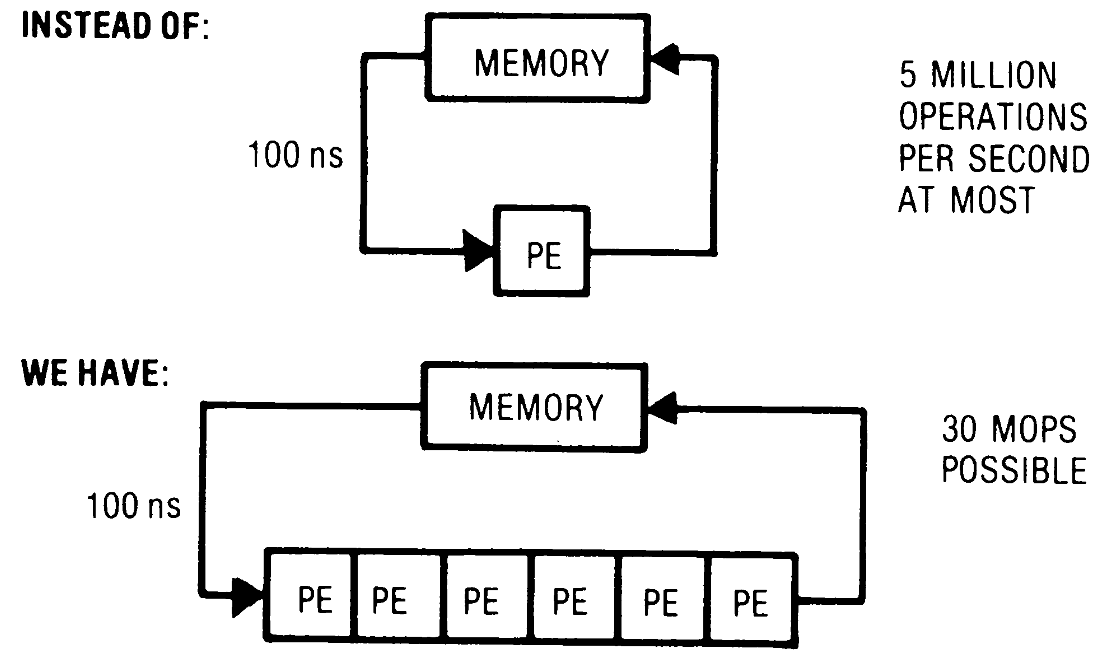
\includegraphics[width=\linewidth]{systolic_array.png}\\[2pt]
{\tiny H.\,T. Kung, \emph{Why systolic architectures?} (1982)}
\end{center}
\end{minipage}\hfill
\begin{minipage}{0.57\textwidth}
\begin{center}
\only<1>{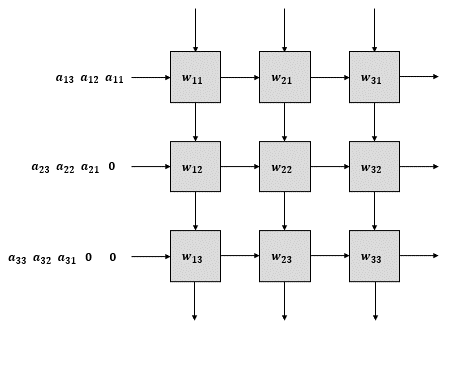
\includegraphics[height=4.1cm]{bench/img/sys_1.png}}%
\only<2>{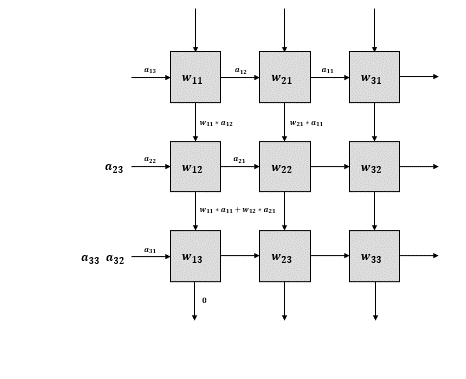
\includegraphics[height=4.1cm]{bench/img/sys_4.png}}%
\only<3>{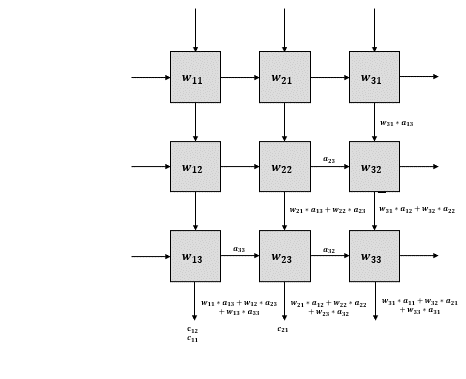
\includegraphics[height=4.1cm]{bench/img/sys_7.png}}%
\only<4>{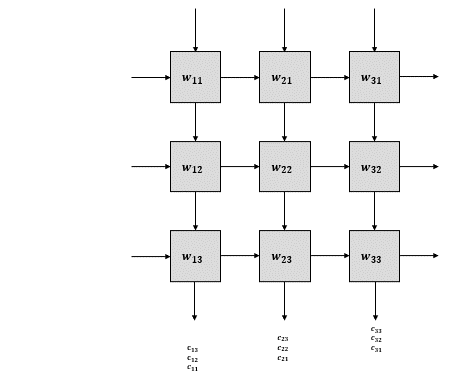
\includegraphics[height=4.1cm]{bench/img/sys_10.png}}\\[2pt]
{\tiny Weight-stationary dataflow: one operand fetch feeds a whole row.}
\end{center}
\end{minipage}

\end{frame}


% =====================================================================
%  Frame "contraintes de l'Edge TPU".
%  Texte reduit au minimum, complementaire de l'oral.
%  Etait la premiere des deux frames de frames_tpu_pruning.tex.
% =====================================================================

\begin{frame}
\frametitle{Edge TPU}
\framesubtitle{Three constraints}

\vspace{0.3cm}

\begin{itemize}\setlength{\itemsep}{14pt}
  \item[{\color{blue!80!black}$\bullet$}]
    \textbf{A fixed set of operations}\\
    {\small Conv, depthwise conv, pooling, add, concat, fully connected.
     The graph is cut at the first unsupported one.}
  \item[{\color{blue!80!black}$\bullet$}]
    \textbf{INT8 only}\\
    {\small Post-training quantization, 100 calibration images.}
  \item[{\color{blue!80!black}$\bullet$}]
    \textbf{8\,MB of on-chip memory}\\
    {\small What does not fit is re-sent at \emph{every} inference,
     $\approx 3.3$\,ms per MB.}
\end{itemize}

\vspace{0.5cm}
\begin{center}
{\color{blue!80!black}\textbf{The lighter the model, the lower its latency.}}
\end{center}

\end{frame}


% =====================================================================
%  Frame "Performance of the edge TPU" : les deux tables de mesures des
%  baselines non elaguees. Etait la slide "Unpruned baselines" de
%  frames_benchmark.tex, remontee juste apres les trois contraintes.
%  \tpuhi : mise en evidence (gras + rouge fonce) des valeurs commentees
%  a l'oral.
% =====================================================================

\newcommand{\tpuhi}[1]{{\color{red!65!black}\textbf{#1}}}

\begin{frame}
\frametitle{Performance of the Edge TPU}

\begin{center}
\setlength{\tabcolsep}{4pt}
\renewcommand{\arraystretch}{0.95}
{\tiny
\begin{tabular}{lrrrrr}
\toprule
\multicolumn{6}{c}{\textbf{Steady-state latency, and model size split between
on-chip SRAM and off-chip memory}}\\
\midrule
Model & CPU (ms) & TPU (ms) & On-chip (MB) & Off-chip (MB) & Speedup \\
\midrule
GoogLeNet      &  63.0 &  2.0 & 5.66 & \tpuhi{0.00}  & \tpuhi{30.9$\times$} \\
WRN-28-10      & 681.5 & 92.1 & 8.00 & 27.13 &  7.4$\times$ \\
ResNet-18      &  74.4 & 11.4 & 8.00 &  2.84 &  6.5$\times$ \\
MobileNetV2    &   9.7 &  1.2 & 2.70 &  0.00 &  7.8$\times$ \\
SqueezeNet 1.1 &   4.6 &  0.7 & 0.83 &  0.00 &  6.9$\times$ \\
ResNet-50      & 188.3 & 50.9 & 8.00 & 15.30 &  3.7$\times$ \\
VGG-19         &  70.7 & 39.3 & 8.00 & \tpuhi{11.30} & \tpuhi{1.8$\times$} \\
\bottomrule
\end{tabular}}

\vspace{0.35cm}

{\tiny
\begin{tabular}{lrrr}
\toprule
\multicolumn{4}{c}{\textbf{Cold start: first vs.\ second inference in a fresh
interpreter}}\\
\midrule
Model & 1st inf.\ (ms) & 2nd inf.\ (ms) & Ratio \\
\midrule
GoogLeNet      &  21.43 &  2.13 & \tpuhi{10.0$\times$} \\
WRN-28-10      & 116.66 & 91.13 &  1.3$\times$ \\
ResNet-18      &  36.94 & 11.51 &  3.2$\times$ \\
MobileNetV2    &  10.97 &  1.34 &  8.2$\times$ \\
SqueezeNet 1.1 &   3.88 &  0.75 &  5.2$\times$ \\
ResNet-50      &  75.62 & 50.23 &  1.5$\times$ \\
VGG-19         &  63.92 & 38.79 &  1.7$\times$ \\
\bottomrule
\end{tabular}}
\end{center}

\end{frame}


% =====================================================================
%  Frame "structured pruning".
%  Etait la seconde des deux frames de frames_tpu_pruning.tex.
% =====================================================================

\begin{frame}
\frametitle{Structured pruning}

\vspace{0.2cm}

{\small
\begin{itemize}\setlength{\itemsep}{7pt}
  \item[{\color{blue!80!black}$\bullet$}]
    There are \textbf{two types of pruning}:
    \begin{itemize}\setlength{\itemsep}{4pt}\setlength{\topsep}{4pt}
      \item[{\color{blue!80!black}--}]
        \emph{Unstructured}: weights become zeros, tensor shapes do not change.
      \item[{\color{blue!80!black}--}]
        \emph{Structured}: whole filters are removed, so the tensors really get
        smaller and the model really gets faster.
        \textbf{We choose this one.}
    \end{itemize}
  \item[{\color{blue!80!black}$\bullet$}]
    The added difficulty is \textbf{dependency tracking}: cutting one filter
    changes the layers it feeds, and residual additions or concatenations tie
    several layers together. All of them must be cut consistently.
  \item[{\color{blue!80!black}$\bullet$}]
    Filters are ranked \textbf{across the whole network}: we set one target for
    the model, and the rate of each layer follows from the ranking.
\end{itemize}}

\vspace{0.3cm}
\begin{center}
\makebox[\linewidth][c]{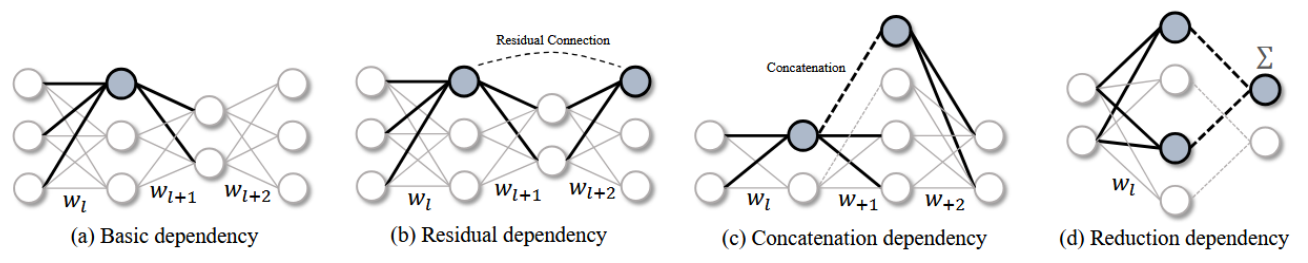
\includegraphics[width=1.0\linewidth]{bench/img/dependencies.png}}
\end{center}

\end{frame}


% =====================================================================
%  Frames "benchmark" : les slides de resultats elagues.
%  A inserer dans presentation_dsd2026.tex par : % =====================================================================
%  Frames "benchmark" : les slides de resultats elagues.
%  A inserer dans presentation_dsd2026.tex par : % =====================================================================
%  Frames "benchmark" : les slides de resultats elagues.
%  A inserer dans presentation_dsd2026.tex par : \input{frames_benchmark}
%  Prerequis (deja dans le preambule) : pgfplots + groupplots, graphicx,
%  booktabs, tikz, xcolor.
%  Donnees : bench/data/*.csv       Images : bench/img/*
%  Les figures sont en pgfplots, meme rendu que les figures de l'article.
% =====================================================================

% --- palette des criteres d'importance (identique a celle de l'article) ---
\definecolor{impmagnitudel1}{HTML}{1F77B4}
\definecolor{impmagnitudel2}{HTML}{AEC7E8}
\definecolor{impbnscale}{HTML}{FF7F0E}
\definecolor{impfpgm}{HTML}{2CA02C}
\definecolor{imptaylor}{HTML}{D62728}
\definecolor{impobdc}{HTML}{9467BD}
\definecolor{imprandom}{HTML}{7F7F7F}

% --- style commun a tous les panneaux ---
\pgfplotsset{
  benchpanel/.style={
    grid=both, grid style={dashed,gray!30},
    tick label style={font=\scriptsize},
    label style={font=\scriptsize},
    title style={font=\small},
  },
  benchcurves/.style={mark=none, line width=1.0pt, unbounded coords=jump},
}

% --- legende partagee (7 criteres), construite une fois par frame ---
\newcommand{\benchlegendcore}[2]{%
\begin{tikzpicture}
\begin{axis}[hide axis, scale only axis, width=1pt, height=1pt,
  xmin=0, xmax=1, ymin=0, ymax=1,
  legend columns=4, legend to name=#1,
  legend style={draw=gray!50, font=\scriptsize, /tikz/every even column/.append style={column sep=6pt}}]
\addplot[draw=none, forget plot] coordinates {(0,0)};
\addlegendimage{color=impmagnitudel1, line width=1.0pt}\addlegendentry{Magnitude L1}
\addlegendimage{color=impmagnitudel2, line width=1.0pt}\addlegendentry{Magnitude L2}
\addlegendimage{color=impbnscale, line width=1.0pt}\addlegendentry{BN-Scale}
\addlegendimage{color=impfpgm, line width=1.0pt}\addlegendentry{FPGM}
\addlegendimage{color=imptaylor, line width=1.0pt}\addlegendentry{Taylor}
\addlegendimage{color=impobdc, line width=1.0pt}\addlegendentry{OBD-C}
\addlegendimage{color=imprandom, line width=1.0pt}\addlegendentry{Random}
#2
\end{axis}
\end{tikzpicture}}
\newcommand{\benchlegend}[1]{\benchlegendcore{#1}{}}
\newcommand{\benchlegendfit}[1]{\benchlegendcore{#1}{%
\addlegendimage{color=red!70!black, dash dot, line width=1.0pt}\addlegendentry{Fits 8\,MB SRAM}}}

% --- les 7 courbes d'un fichier CSV (colonnes <crit>_x / <crit>_y) ---
\newcommand{\benchseven}[1]{%
\addplot[benchcurves, color=impmagnitudel1] table[x=magl1_x,   y=magl1_y,   col sep=comma] {#1};
\addplot[benchcurves, color=impmagnitudel2] table[x=magl2_x,   y=magl2_y,   col sep=comma] {#1};
\addplot[benchcurves, color=impbnscale]     table[x=bnscale_x, y=bnscale_y, col sep=comma] {#1};
\addplot[benchcurves, color=impfpgm]        table[x=fpgm_x,    y=fpgm_y,    col sep=comma] {#1};
\addplot[benchcurves, color=imptaylor]      table[x=taylor_x,  y=taylor_y,  col sep=comma] {#1};
\addplot[benchcurves, color=impobdc]        table[x=obdc_x,    y=obdc_y,    col sep=comma] {#1};
\addplot[benchcurves, color=imprandom]      table[x=random_x,  y=random_y,  col sep=comma] {#1};}


% =====================================================================
\section{Measurement study}
% =====================================================================

% ------------------------------ SLIDE 6 ------------------------------
\begin{frame}
\frametitle{Benchmark on the Coral USB Edge TPU}

\vspace{0.15cm}

\begin{minipage}[t]{0.48\textwidth}\vspace{0pt}
{\scriptsize
\setlength{\tabcolsep}{4pt}
\begin{tabularx}{\linewidth}{@{}l >{\raggedright\arraybackslash}X@{}}
\toprule
\multicolumn{2}{c}{\textbf{7 architectures, by topology}}\\
\midrule
Sequential        & VGG-19 \\
Residual          & ResNet-18, ResNet-50, WRN-28-10 \\
Inverted residual & MobileNetV2 \\
Concatenation     & GoogLeNet, SqueezeNet 1.1 \\
\bottomrule
\end{tabularx}}
\end{minipage}\hfill
\begin{minipage}[t]{0.48\textwidth}\vspace{0pt}
{\scriptsize
\setlength{\tabcolsep}{4pt}
\begin{tabularx}{\linewidth}{@{}l >{\raggedright\arraybackslash}X@{}}
\toprule
\multicolumn{2}{c}{\textbf{7 criteria, by information used}}\\
\midrule
Data-free \,{\tiny(weights)}   & Magnitude L1, L2, FPGM \\
Sparsity learning              & BN-Scale \\
Data-driven \,{\tiny(fwd+bwd)} & Taylor, OBD-C \\
Control                        & Random \\
\bottomrule
\end{tabularx}}
\end{minipage}

\vspace{0.4cm}

\begin{minipage}[c]{0.58\textwidth}
{\small
\begin{itemize}\setlength{\itemsep}{8pt}
  \item[{\color{blue!80!black}$\bullet$}]
    \textbf{9 compression rates}\\
    10\,\% to 90\,\% of parameters removed, in steps of 10.
  \item[{\color{blue!80!black}$\bullet$}]
    \textbf{PruningBench protocol}~[1]\\
    Unchanged: 400 iterative steps, global ranking, 100 recovery epochs.\\
    {\scriptsize 404 of the 441 combinations reached the accelerator.}
\end{itemize}}
\end{minipage}\hfill
\begin{minipage}[c]{0.38\textwidth}
\begin{center}
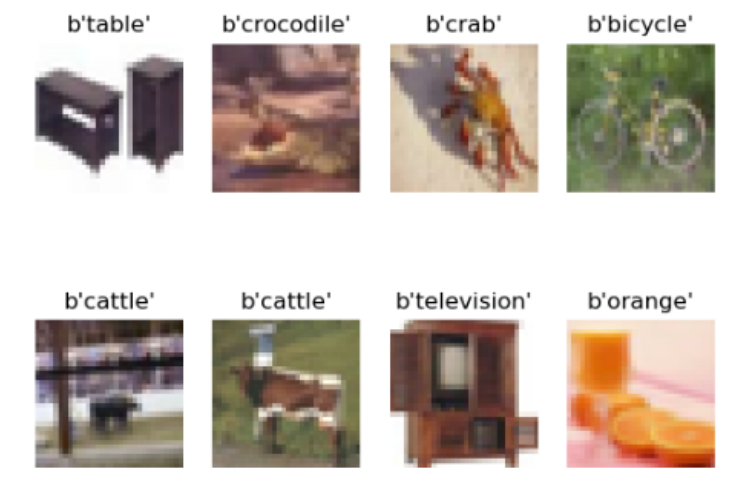
\includegraphics[width=\linewidth]{bench/img/cifar100.png}\\[3pt]
{\scriptsize CIFAR-100, 100 classes, 32$\times$32}
\end{center}
\end{minipage}

\begin{thebibliography}{10}
\beamertemplatearticlebibitems
\tiny
\bibitem{PruningBench} C. Li \emph{et al.}, A Comprehensive Study of Structural
Pruning for Vision Models (2025)
\end{thebibliography}

\end{frame}


% ------------------------------ SLIDE 7 ------------------------------
\begin{frame}
\frametitle{Latency of the pruned models}
\framesubtitle{Edge TPU speed-up versus parameter reduction, and INT8 model size}

\benchlegendfit{leg:benchspeedup}

\begin{center}
\makebox[\linewidth][c]{%
\begin{tikzpicture}
\begin{axis}[benchpanel, scale only axis, width=2.5cm, height=2.5cm, name=pVGG,
  title={VGG-19}, title style={font=\small, yshift=0.62cm},
  xlabel={Parameter reduction (\%)},
  ylabel={Edge TPU speed-up ($\times$)},
  xmin=0, xmax=90, xtick={0,30,60,90}, enlarge x limits=false]
\addplot[mark=none, domain=0:90, samples=2, dashed, black, thin] {1};
\benchseven{bench/data/sp_vgg19.csv}
\draw[red!70!black, dash dot, thick] ({axis cs:58.76,0}|-{rel axis cs:0,0}) -- ({axis cs:58.76,0}|-{rel axis cs:0,1});
\end{axis}
\begin{axis}[scale only axis, width=2.5cm, height=2.5cm,
  at=(pVGG.south west), anchor=south west,
  axis x line*=top, axis y line=none, ytick=\empty, ymin=0, ymax=1,
  xmin=1.93, xmax=19.30, x dir=reverse, enlarge x limits=false,
  xtick={2,6,10,14,18}, tick label style={font=\scriptsize},
  xlabel={INT8 size (MB)}, label style={font=\scriptsize}]
\end{axis}
\end{tikzpicture}\hspace{0.3cm}
\begin{tikzpicture}
\begin{axis}[benchpanel, scale only axis, width=2.5cm, height=2.5cm, name=pR18,
  title={ResNet-18}, title style={font=\small, yshift=0.62cm},
  xlabel={Parameter reduction (\%)},
  xmin=0, xmax=90, xtick={0,30,60,90}, enlarge x limits=false]
\addplot[mark=none, domain=0:90, samples=2, dashed, black, thin] {1};
\benchseven{bench/data/sp_resnet18.csv}
\draw[red!70!black, dash dot, thick] ({axis cs:26.29,0}|-{rel axis cs:0,0}) -- ({axis cs:26.29,0}|-{rel axis cs:0,1});
\end{axis}
\begin{axis}[scale only axis, width=2.5cm, height=2.5cm,
  at=(pR18.south west), anchor=south west,
  axis x line*=top, axis y line=none, ytick=\empty, ymin=0, ymax=1,
  xmin=1.08, xmax=10.84, x dir=reverse, enlarge x limits=false,
  xtick={2,4,6,8,10}, tick label style={font=\scriptsize},
  xlabel={INT8 size (MB)}, label style={font=\scriptsize}]
\end{axis}
\end{tikzpicture}\hspace{0.3cm}
\begin{tikzpicture}
\begin{axis}[benchpanel, scale only axis, width=2.5cm, height=2.5cm, name=pGLN,
  title={GoogLeNet}, title style={font=\small, yshift=0.62cm},
  xlabel={Parameter reduction (\%)},
  xmin=0, xmax=90, xtick={0,30,60,90}, enlarge x limits=false]
\addplot[mark=none, domain=0:90, samples=2, dashed, black, thin] {1};
\benchseven{bench/data/sp_googlenet.csv}
\end{axis}
\begin{axis}[scale only axis, width=2.5cm, height=2.5cm,
  at=(pGLN.south west), anchor=south west,
  axis x line*=top, axis y line=none, ytick=\empty, ymin=0, ymax=1,
  xmin=0.57, xmax=5.66, x dir=reverse, enlarge x limits=false,
  xtick={1,2,3,4,5}, tick label style={font=\scriptsize},
  xlabel={INT8 size (MB)}, label style={font=\scriptsize}]
\end{axis}
\end{tikzpicture}}

\vspace{3pt}
\ref{leg:benchspeedup}

\vspace{3pt}
{\small Red line: the rate at which the model first fits entirely on chip.
Note that each panel has its own vertical scale.}
\end{center}

\end{frame}


% ------------------------------ SLIDE 8 ------------------------------
\begin{frame}
\frametitle{Accuracy}
\framesubtitle{ResNet-18: accuracy right after pruning, and recovery fine-tuning}

\benchlegend{leg:benchacc}

\begin{center}
\makebox[\linewidth][c]{%
\begin{tikzpicture}
\begin{groupplot}[
  group style={group size=2 by 1, horizontal sep=1.5cm},
  benchpanel, scale only axis, width=3.1cm, height=3.1cm,
  title style={font=\small}]

\nextgroupplot[title={After pruning, before FT},
               xlabel={Pruning target (\%)}, ylabel={Top-1 val.\ acc.\ (\%)},
               xtick={10,30,50,70,90}]
\addplot[mark=none, domain=10:90, samples=2, dashed, black, thin] {76.890};
\benchseven{bench/data/pp_resnet18.csv}

\nextgroupplot[title={Recovery FT at 90\,\%},
               xlabel={Epoch}, ylabel={Top-1 val.\ acc.\ (\%)},
               xtick={0,50,100}]
\addplot[mark=none, domain=0:100, samples=2, dashed, black, thin, forget plot] {76.890};
\addplot[benchcurves, color=impmagnitudel1] table[x=epoch, y=magnitude_l1, col sep=comma] {bench/data/ft_resnet18_90.csv};
\addplot[benchcurves, color=impmagnitudel2] table[x=epoch, y=magnitude_l2, col sep=comma] {bench/data/ft_resnet18_90.csv};
\addplot[benchcurves, color=impbnscale]     table[x=epoch, y=bn_scale,     col sep=comma] {bench/data/ft_resnet18_90.csv};
\addplot[benchcurves, color=impfpgm]        table[x=epoch, y=fpgm,         col sep=comma] {bench/data/ft_resnet18_90.csv};
\addplot[benchcurves, color=imptaylor]      table[x=epoch, y=taylor,       col sep=comma] {bench/data/ft_resnet18_90.csv};
\addplot[benchcurves, color=impobdc]        table[x=epoch, y=obdc,         col sep=comma] {bench/data/ft_resnet18_90.csv};
\addplot[benchcurves, color=imprandom]      table[x=epoch, y=random,       col sep=comma] {bench/data/ft_resnet18_90.csv};

\end{groupplot}
\end{tikzpicture}}

\vspace{3pt}
\ref{leg:benchacc}

\vspace{3pt}
{\small Dashed line: unpruned baseline. Both indicators give the same ranking.}
\end{center}

\end{frame}


% ------------------------------ SLIDE 9 -----------------------------
\begin{frame}
\frametitle{Accuracy and latency disagree}
\framesubtitle{ResNet-50: the criterion that best preserves accuracy is the slowest}

\benchlegendfit{leg:benchboth}

\begin{center}
\makebox[\linewidth][c]{%
\begin{tikzpicture}
\begin{groupplot}[
  group style={group size=2 by 1, horizontal sep=1.5cm},
  benchpanel, scale only axis, width=3.1cm, height=3.1cm,
  title style={font=\small},
  xlabel={Parameter reduction (\%)}]

\nextgroupplot[title={Accuracy right after pruning},
               ylabel={Top-1 val.\ acc.\ (\%)}]
\addplot[mark=none, domain=10:90, samples=2, dashed, black, thin] {77.810};
\benchseven{bench/data/pp_resnet50.csv}

\nextgroupplot[title={Edge TPU speed-up}, ylabel={Speed-up ($\times$)}]
\addplot[mark=none, domain=0:90, samples=2, dashed, black, thin] {1};
\benchseven{bench/data/sp_resnet50.csv}
\draw[red!70!black, dash dot, thick] ({axis cs:65.90,0}|-{rel axis cs:0,0}) -- ({axis cs:65.90,0}|-{rel axis cs:0,1});

\end{groupplot}
\end{tikzpicture}}

\vspace{2pt}
\ref{leg:benchboth}

\vspace{2pt}
{\small At equal parameter reduction, two criteria do not produce the same
on-chip footprint: \emph{where} channels are removed matters.}
\end{center}

\end{frame}


% ------------------------------ SLIDE 10 -----------------------------
\begin{frame}
\frametitle{Real-time scheduling of multiple DNNs on a single TPU}
\framesubtitle{Illustrative use case}

\begin{minipage}{0.64\textwidth}
{\small
\begin{itemize}\setlength{\itemsep}{3pt}
  \item[{\color{blue!80!black}$\bullet$}] Single TPU
  \item[{\color{blue!80!black}$\bullet$}] Many DNNs executed at different rates
  \item[{\color{blue!80!black}$\bullet$}] \emph{Earliest Deadline First (EDF)}
  \item[{\color{blue!80!black}$\bullet$}] Non-preemptive avoids weight reloading
  \item[{\color{blue!80!black}$\bullet$}] Sporadic tasks (\emph{i.e.,} event-triggered)
\end{itemize}}

\vspace{0.25cm}

\setlength{\tabcolsep}{4pt}
\renewcommand{\arraystretch}{0.95}
{\tiny
\begin{tabular}{llrrr}
\toprule
Function & Model & $T$ (ms) & $C$ (ms) & $C/T$ \\
\midrule
Nozzle trigger    & ResNet-18    &  20 & 11.4 & 0.57 \\
Crop growth stage & MobileNetV2  &  33 &  1.2 & 0.04 \\
Weed species      & ResNet-50    & 100 & 50.9 & 0.51 \\
Ground cover      & VGG-19       & 200 & 39.3 & 0.20 \\
\midrule
\multicolumn{4}{r}{Total utilization} & \textbf{\color{red!80!black}1.32} \\
\bottomrule
\end{tabular}}

\vspace{0.2cm}
{\small \color{red!80!black}$U > 1$ : the task set is \textbf{infeasible}.}
\end{minipage}\hfill
\begin{minipage}{0.32\textwidth}
\begin{center}
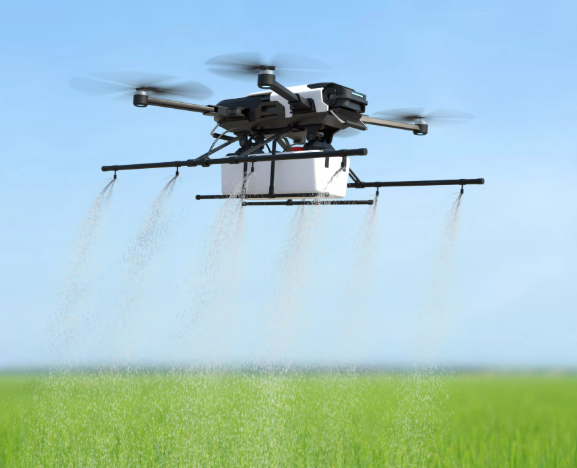
\includegraphics[width=\linewidth]{bench/img/drone_rampe_de_buses.png}\\[5pt]
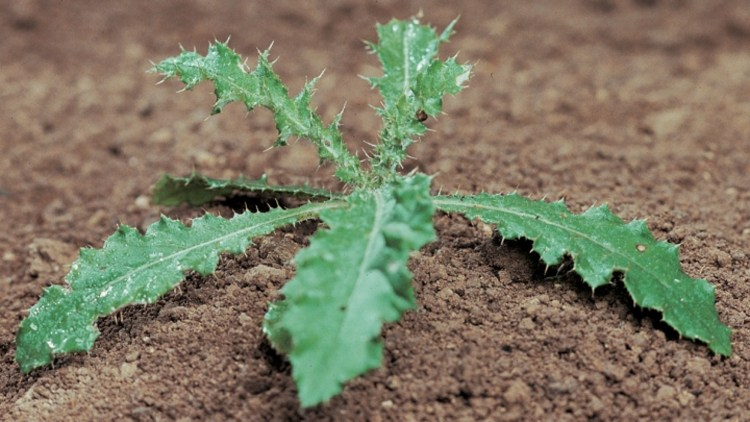
\includegraphics[width=\linewidth]{bench/img/adventice.jpg}
\end{center}
\end{minipage}

\vspace{0.2cm}

\begin{thebibliography}{10}
\beamertemplatearticlebibitems
\tiny
\bibitem{Buttazzo} G. Buttazzo, Can We Trust AI-Powered Real-Time Embedded
Systems? NG-RES (2022)
\end{thebibliography}

\end{frame}

%  Prerequis (deja dans le preambule) : pgfplots + groupplots, graphicx,
%  booktabs, tikz, xcolor.
%  Donnees : bench/data/*.csv       Images : bench/img/*
%  Les figures sont en pgfplots, meme rendu que les figures de l'article.
% =====================================================================

% --- palette des criteres d'importance (identique a celle de l'article) ---
\definecolor{impmagnitudel1}{HTML}{1F77B4}
\definecolor{impmagnitudel2}{HTML}{AEC7E8}
\definecolor{impbnscale}{HTML}{FF7F0E}
\definecolor{impfpgm}{HTML}{2CA02C}
\definecolor{imptaylor}{HTML}{D62728}
\definecolor{impobdc}{HTML}{9467BD}
\definecolor{imprandom}{HTML}{7F7F7F}

% --- style commun a tous les panneaux ---
\pgfplotsset{
  benchpanel/.style={
    grid=both, grid style={dashed,gray!30},
    tick label style={font=\scriptsize},
    label style={font=\scriptsize},
    title style={font=\small},
  },
  benchcurves/.style={mark=none, line width=1.0pt, unbounded coords=jump},
}

% --- legende partagee (7 criteres), construite une fois par frame ---
\newcommand{\benchlegendcore}[2]{%
\begin{tikzpicture}
\begin{axis}[hide axis, scale only axis, width=1pt, height=1pt,
  xmin=0, xmax=1, ymin=0, ymax=1,
  legend columns=4, legend to name=#1,
  legend style={draw=gray!50, font=\scriptsize, /tikz/every even column/.append style={column sep=6pt}}]
\addplot[draw=none, forget plot] coordinates {(0,0)};
\addlegendimage{color=impmagnitudel1, line width=1.0pt}\addlegendentry{Magnitude L1}
\addlegendimage{color=impmagnitudel2, line width=1.0pt}\addlegendentry{Magnitude L2}
\addlegendimage{color=impbnscale, line width=1.0pt}\addlegendentry{BN-Scale}
\addlegendimage{color=impfpgm, line width=1.0pt}\addlegendentry{FPGM}
\addlegendimage{color=imptaylor, line width=1.0pt}\addlegendentry{Taylor}
\addlegendimage{color=impobdc, line width=1.0pt}\addlegendentry{OBD-C}
\addlegendimage{color=imprandom, line width=1.0pt}\addlegendentry{Random}
#2
\end{axis}
\end{tikzpicture}}
\newcommand{\benchlegend}[1]{\benchlegendcore{#1}{}}
\newcommand{\benchlegendfit}[1]{\benchlegendcore{#1}{%
\addlegendimage{color=red!70!black, dash dot, line width=1.0pt}\addlegendentry{Fits 8\,MB SRAM}}}

% --- les 7 courbes d'un fichier CSV (colonnes <crit>_x / <crit>_y) ---
\newcommand{\benchseven}[1]{%
\addplot[benchcurves, color=impmagnitudel1] table[x=magl1_x,   y=magl1_y,   col sep=comma] {#1};
\addplot[benchcurves, color=impmagnitudel2] table[x=magl2_x,   y=magl2_y,   col sep=comma] {#1};
\addplot[benchcurves, color=impbnscale]     table[x=bnscale_x, y=bnscale_y, col sep=comma] {#1};
\addplot[benchcurves, color=impfpgm]        table[x=fpgm_x,    y=fpgm_y,    col sep=comma] {#1};
\addplot[benchcurves, color=imptaylor]      table[x=taylor_x,  y=taylor_y,  col sep=comma] {#1};
\addplot[benchcurves, color=impobdc]        table[x=obdc_x,    y=obdc_y,    col sep=comma] {#1};
\addplot[benchcurves, color=imprandom]      table[x=random_x,  y=random_y,  col sep=comma] {#1};}


% =====================================================================
\section{Measurement study}
% =====================================================================

% ------------------------------ SLIDE 6 ------------------------------
\begin{frame}
\frametitle{Benchmark on the Coral USB Edge TPU}

\vspace{0.15cm}

\begin{minipage}[t]{0.48\textwidth}\vspace{0pt}
{\scriptsize
\setlength{\tabcolsep}{4pt}
\begin{tabularx}{\linewidth}{@{}l >{\raggedright\arraybackslash}X@{}}
\toprule
\multicolumn{2}{c}{\textbf{7 architectures, by topology}}\\
\midrule
Sequential        & VGG-19 \\
Residual          & ResNet-18, ResNet-50, WRN-28-10 \\
Inverted residual & MobileNetV2 \\
Concatenation     & GoogLeNet, SqueezeNet 1.1 \\
\bottomrule
\end{tabularx}}
\end{minipage}\hfill
\begin{minipage}[t]{0.48\textwidth}\vspace{0pt}
{\scriptsize
\setlength{\tabcolsep}{4pt}
\begin{tabularx}{\linewidth}{@{}l >{\raggedright\arraybackslash}X@{}}
\toprule
\multicolumn{2}{c}{\textbf{7 criteria, by information used}}\\
\midrule
Data-free \,{\tiny(weights)}   & Magnitude L1, L2, FPGM \\
Sparsity learning              & BN-Scale \\
Data-driven \,{\tiny(fwd+bwd)} & Taylor, OBD-C \\
Control                        & Random \\
\bottomrule
\end{tabularx}}
\end{minipage}

\vspace{0.4cm}

\begin{minipage}[c]{0.58\textwidth}
{\small
\begin{itemize}\setlength{\itemsep}{8pt}
  \item[{\color{blue!80!black}$\bullet$}]
    \textbf{9 compression rates}\\
    10\,\% to 90\,\% of parameters removed, in steps of 10.
  \item[{\color{blue!80!black}$\bullet$}]
    \textbf{PruningBench protocol}~[1]\\
    Unchanged: 400 iterative steps, global ranking, 100 recovery epochs.\\
    {\scriptsize 404 of the 441 combinations reached the accelerator.}
\end{itemize}}
\end{minipage}\hfill
\begin{minipage}[c]{0.38\textwidth}
\begin{center}
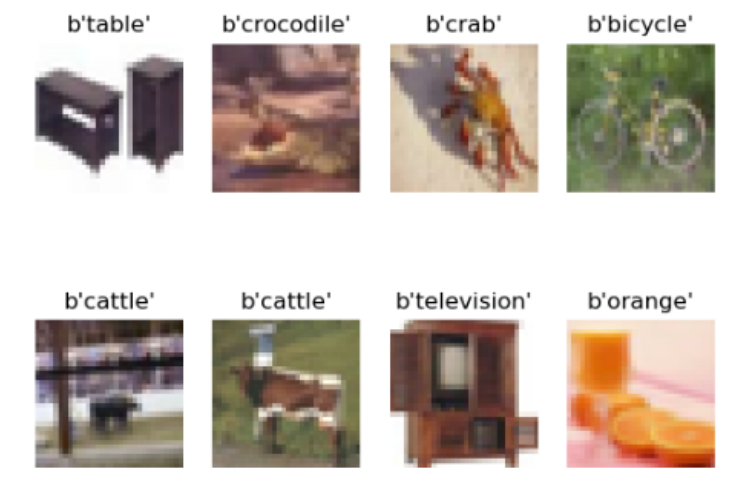
\includegraphics[width=\linewidth]{bench/img/cifar100.png}\\[3pt]
{\scriptsize CIFAR-100, 100 classes, 32$\times$32}
\end{center}
\end{minipage}

\begin{thebibliography}{10}
\beamertemplatearticlebibitems
\tiny
\bibitem{PruningBench} C. Li \emph{et al.}, A Comprehensive Study of Structural
Pruning for Vision Models (2025)
\end{thebibliography}

\end{frame}


% ------------------------------ SLIDE 7 ------------------------------
\begin{frame}
\frametitle{Latency of the pruned models}
\framesubtitle{Edge TPU speed-up versus parameter reduction, and INT8 model size}

\benchlegendfit{leg:benchspeedup}

\begin{center}
\makebox[\linewidth][c]{%
\begin{tikzpicture}
\begin{axis}[benchpanel, scale only axis, width=2.5cm, height=2.5cm, name=pVGG,
  title={VGG-19}, title style={font=\small, yshift=0.62cm},
  xlabel={Parameter reduction (\%)},
  ylabel={Edge TPU speed-up ($\times$)},
  xmin=0, xmax=90, xtick={0,30,60,90}, enlarge x limits=false]
\addplot[mark=none, domain=0:90, samples=2, dashed, black, thin] {1};
\benchseven{bench/data/sp_vgg19.csv}
\draw[red!70!black, dash dot, thick] ({axis cs:58.76,0}|-{rel axis cs:0,0}) -- ({axis cs:58.76,0}|-{rel axis cs:0,1});
\end{axis}
\begin{axis}[scale only axis, width=2.5cm, height=2.5cm,
  at=(pVGG.south west), anchor=south west,
  axis x line*=top, axis y line=none, ytick=\empty, ymin=0, ymax=1,
  xmin=1.93, xmax=19.30, x dir=reverse, enlarge x limits=false,
  xtick={2,6,10,14,18}, tick label style={font=\scriptsize},
  xlabel={INT8 size (MB)}, label style={font=\scriptsize}]
\end{axis}
\end{tikzpicture}\hspace{0.3cm}
\begin{tikzpicture}
\begin{axis}[benchpanel, scale only axis, width=2.5cm, height=2.5cm, name=pR18,
  title={ResNet-18}, title style={font=\small, yshift=0.62cm},
  xlabel={Parameter reduction (\%)},
  xmin=0, xmax=90, xtick={0,30,60,90}, enlarge x limits=false]
\addplot[mark=none, domain=0:90, samples=2, dashed, black, thin] {1};
\benchseven{bench/data/sp_resnet18.csv}
\draw[red!70!black, dash dot, thick] ({axis cs:26.29,0}|-{rel axis cs:0,0}) -- ({axis cs:26.29,0}|-{rel axis cs:0,1});
\end{axis}
\begin{axis}[scale only axis, width=2.5cm, height=2.5cm,
  at=(pR18.south west), anchor=south west,
  axis x line*=top, axis y line=none, ytick=\empty, ymin=0, ymax=1,
  xmin=1.08, xmax=10.84, x dir=reverse, enlarge x limits=false,
  xtick={2,4,6,8,10}, tick label style={font=\scriptsize},
  xlabel={INT8 size (MB)}, label style={font=\scriptsize}]
\end{axis}
\end{tikzpicture}\hspace{0.3cm}
\begin{tikzpicture}
\begin{axis}[benchpanel, scale only axis, width=2.5cm, height=2.5cm, name=pGLN,
  title={GoogLeNet}, title style={font=\small, yshift=0.62cm},
  xlabel={Parameter reduction (\%)},
  xmin=0, xmax=90, xtick={0,30,60,90}, enlarge x limits=false]
\addplot[mark=none, domain=0:90, samples=2, dashed, black, thin] {1};
\benchseven{bench/data/sp_googlenet.csv}
\end{axis}
\begin{axis}[scale only axis, width=2.5cm, height=2.5cm,
  at=(pGLN.south west), anchor=south west,
  axis x line*=top, axis y line=none, ytick=\empty, ymin=0, ymax=1,
  xmin=0.57, xmax=5.66, x dir=reverse, enlarge x limits=false,
  xtick={1,2,3,4,5}, tick label style={font=\scriptsize},
  xlabel={INT8 size (MB)}, label style={font=\scriptsize}]
\end{axis}
\end{tikzpicture}}

\vspace{3pt}
\ref{leg:benchspeedup}

\vspace{3pt}
{\small Red line: the rate at which the model first fits entirely on chip.
Note that each panel has its own vertical scale.}
\end{center}

\end{frame}


% ------------------------------ SLIDE 8 ------------------------------
\begin{frame}
\frametitle{Accuracy}
\framesubtitle{ResNet-18: accuracy right after pruning, and recovery fine-tuning}

\benchlegend{leg:benchacc}

\begin{center}
\makebox[\linewidth][c]{%
\begin{tikzpicture}
\begin{groupplot}[
  group style={group size=2 by 1, horizontal sep=1.5cm},
  benchpanel, scale only axis, width=3.1cm, height=3.1cm,
  title style={font=\small}]

\nextgroupplot[title={After pruning, before FT},
               xlabel={Pruning target (\%)}, ylabel={Top-1 val.\ acc.\ (\%)},
               xtick={10,30,50,70,90}]
\addplot[mark=none, domain=10:90, samples=2, dashed, black, thin] {76.890};
\benchseven{bench/data/pp_resnet18.csv}

\nextgroupplot[title={Recovery FT at 90\,\%},
               xlabel={Epoch}, ylabel={Top-1 val.\ acc.\ (\%)},
               xtick={0,50,100}]
\addplot[mark=none, domain=0:100, samples=2, dashed, black, thin, forget plot] {76.890};
\addplot[benchcurves, color=impmagnitudel1] table[x=epoch, y=magnitude_l1, col sep=comma] {bench/data/ft_resnet18_90.csv};
\addplot[benchcurves, color=impmagnitudel2] table[x=epoch, y=magnitude_l2, col sep=comma] {bench/data/ft_resnet18_90.csv};
\addplot[benchcurves, color=impbnscale]     table[x=epoch, y=bn_scale,     col sep=comma] {bench/data/ft_resnet18_90.csv};
\addplot[benchcurves, color=impfpgm]        table[x=epoch, y=fpgm,         col sep=comma] {bench/data/ft_resnet18_90.csv};
\addplot[benchcurves, color=imptaylor]      table[x=epoch, y=taylor,       col sep=comma] {bench/data/ft_resnet18_90.csv};
\addplot[benchcurves, color=impobdc]        table[x=epoch, y=obdc,         col sep=comma] {bench/data/ft_resnet18_90.csv};
\addplot[benchcurves, color=imprandom]      table[x=epoch, y=random,       col sep=comma] {bench/data/ft_resnet18_90.csv};

\end{groupplot}
\end{tikzpicture}}

\vspace{3pt}
\ref{leg:benchacc}

\vspace{3pt}
{\small Dashed line: unpruned baseline. Both indicators give the same ranking.}
\end{center}

\end{frame}


% ------------------------------ SLIDE 9 -----------------------------
\begin{frame}
\frametitle{Accuracy and latency disagree}
\framesubtitle{ResNet-50: the criterion that best preserves accuracy is the slowest}

\benchlegendfit{leg:benchboth}

\begin{center}
\makebox[\linewidth][c]{%
\begin{tikzpicture}
\begin{groupplot}[
  group style={group size=2 by 1, horizontal sep=1.5cm},
  benchpanel, scale only axis, width=3.1cm, height=3.1cm,
  title style={font=\small},
  xlabel={Parameter reduction (\%)}]

\nextgroupplot[title={Accuracy right after pruning},
               ylabel={Top-1 val.\ acc.\ (\%)}]
\addplot[mark=none, domain=10:90, samples=2, dashed, black, thin] {77.810};
\benchseven{bench/data/pp_resnet50.csv}

\nextgroupplot[title={Edge TPU speed-up}, ylabel={Speed-up ($\times$)}]
\addplot[mark=none, domain=0:90, samples=2, dashed, black, thin] {1};
\benchseven{bench/data/sp_resnet50.csv}
\draw[red!70!black, dash dot, thick] ({axis cs:65.90,0}|-{rel axis cs:0,0}) -- ({axis cs:65.90,0}|-{rel axis cs:0,1});

\end{groupplot}
\end{tikzpicture}}

\vspace{2pt}
\ref{leg:benchboth}

\vspace{2pt}
{\small At equal parameter reduction, two criteria do not produce the same
on-chip footprint: \emph{where} channels are removed matters.}
\end{center}

\end{frame}


% ------------------------------ SLIDE 10 -----------------------------
\begin{frame}
\frametitle{Real-time scheduling of multiple DNNs on a single TPU}
\framesubtitle{Illustrative use case}

\begin{minipage}{0.64\textwidth}
{\small
\begin{itemize}\setlength{\itemsep}{3pt}
  \item[{\color{blue!80!black}$\bullet$}] Single TPU
  \item[{\color{blue!80!black}$\bullet$}] Many DNNs executed at different rates
  \item[{\color{blue!80!black}$\bullet$}] \emph{Earliest Deadline First (EDF)}
  \item[{\color{blue!80!black}$\bullet$}] Non-preemptive avoids weight reloading
  \item[{\color{blue!80!black}$\bullet$}] Sporadic tasks (\emph{i.e.,} event-triggered)
\end{itemize}}

\vspace{0.25cm}

\setlength{\tabcolsep}{4pt}
\renewcommand{\arraystretch}{0.95}
{\tiny
\begin{tabular}{llrrr}
\toprule
Function & Model & $T$ (ms) & $C$ (ms) & $C/T$ \\
\midrule
Nozzle trigger    & ResNet-18    &  20 & 11.4 & 0.57 \\
Crop growth stage & MobileNetV2  &  33 &  1.2 & 0.04 \\
Weed species      & ResNet-50    & 100 & 50.9 & 0.51 \\
Ground cover      & VGG-19       & 200 & 39.3 & 0.20 \\
\midrule
\multicolumn{4}{r}{Total utilization} & \textbf{\color{red!80!black}1.32} \\
\bottomrule
\end{tabular}}

\vspace{0.2cm}
{\small \color{red!80!black}$U > 1$ : the task set is \textbf{infeasible}.}
\end{minipage}\hfill
\begin{minipage}{0.32\textwidth}
\begin{center}
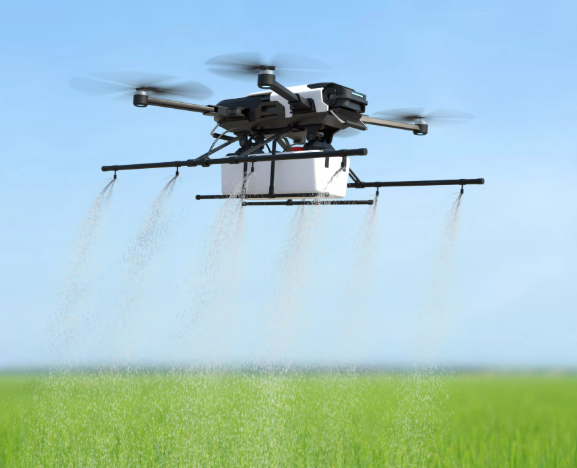
\includegraphics[width=\linewidth]{bench/img/drone_rampe_de_buses.png}\\[5pt]
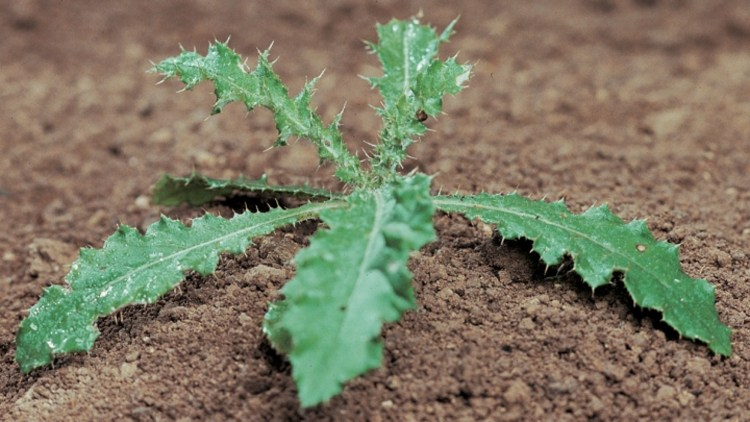
\includegraphics[width=\linewidth]{bench/img/adventice.jpg}
\end{center}
\end{minipage}

\vspace{0.2cm}

\begin{thebibliography}{10}
\beamertemplatearticlebibitems
\tiny
\bibitem{Buttazzo} G. Buttazzo, Can We Trust AI-Powered Real-Time Embedded
Systems? NG-RES (2022)
\end{thebibliography}

\end{frame}

%  Prerequis (deja dans le preambule) : pgfplots + groupplots, graphicx,
%  booktabs, tikz, xcolor.
%  Donnees : bench/data/*.csv       Images : bench/img/*
%  Les figures sont en pgfplots, meme rendu que les figures de l'article.
% =====================================================================

% --- palette des criteres d'importance (identique a celle de l'article) ---
\definecolor{impmagnitudel1}{HTML}{1F77B4}
\definecolor{impmagnitudel2}{HTML}{AEC7E8}
\definecolor{impbnscale}{HTML}{FF7F0E}
\definecolor{impfpgm}{HTML}{2CA02C}
\definecolor{imptaylor}{HTML}{D62728}
\definecolor{impobdc}{HTML}{9467BD}
\definecolor{imprandom}{HTML}{7F7F7F}

% --- style commun a tous les panneaux ---
\pgfplotsset{
  benchpanel/.style={
    grid=both, grid style={dashed,gray!30},
    tick label style={font=\scriptsize},
    label style={font=\scriptsize},
    title style={font=\small},
  },
  benchcurves/.style={mark=none, line width=1.0pt, unbounded coords=jump},
}

% --- legende partagee (7 criteres), construite une fois par frame ---
\newcommand{\benchlegendcore}[2]{%
\begin{tikzpicture}
\begin{axis}[hide axis, scale only axis, width=1pt, height=1pt,
  xmin=0, xmax=1, ymin=0, ymax=1,
  legend columns=4, legend to name=#1,
  legend style={draw=gray!50, font=\scriptsize, /tikz/every even column/.append style={column sep=6pt}}]
\addplot[draw=none, forget plot] coordinates {(0,0)};
\addlegendimage{color=impmagnitudel1, line width=1.0pt}\addlegendentry{Magnitude L1}
\addlegendimage{color=impmagnitudel2, line width=1.0pt}\addlegendentry{Magnitude L2}
\addlegendimage{color=impbnscale, line width=1.0pt}\addlegendentry{BN-Scale}
\addlegendimage{color=impfpgm, line width=1.0pt}\addlegendentry{FPGM}
\addlegendimage{color=imptaylor, line width=1.0pt}\addlegendentry{Taylor}
\addlegendimage{color=impobdc, line width=1.0pt}\addlegendentry{OBD-C}
\addlegendimage{color=imprandom, line width=1.0pt}\addlegendentry{Random}
#2
\end{axis}
\end{tikzpicture}}
\newcommand{\benchlegend}[1]{\benchlegendcore{#1}{}}
\newcommand{\benchlegendfit}[1]{\benchlegendcore{#1}{%
\addlegendimage{color=red!70!black, dash dot, line width=1.0pt}\addlegendentry{Fits 8\,MB SRAM}}}

% --- les 7 courbes d'un fichier CSV (colonnes <crit>_x / <crit>_y) ---
\newcommand{\benchseven}[1]{%
\addplot[benchcurves, color=impmagnitudel1] table[x=magl1_x,   y=magl1_y,   col sep=comma] {#1};
\addplot[benchcurves, color=impmagnitudel2] table[x=magl2_x,   y=magl2_y,   col sep=comma] {#1};
\addplot[benchcurves, color=impbnscale]     table[x=bnscale_x, y=bnscale_y, col sep=comma] {#1};
\addplot[benchcurves, color=impfpgm]        table[x=fpgm_x,    y=fpgm_y,    col sep=comma] {#1};
\addplot[benchcurves, color=imptaylor]      table[x=taylor_x,  y=taylor_y,  col sep=comma] {#1};
\addplot[benchcurves, color=impobdc]        table[x=obdc_x,    y=obdc_y,    col sep=comma] {#1};
\addplot[benchcurves, color=imprandom]      table[x=random_x,  y=random_y,  col sep=comma] {#1};}


% =====================================================================
\section{Measurement study}
% =====================================================================

% ------------------------------ SLIDE 6 ------------------------------
\begin{frame}
\frametitle{Benchmark on the Coral USB Edge TPU}

\vspace{0.15cm}

\begin{minipage}[t]{0.48\textwidth}\vspace{0pt}
{\scriptsize
\setlength{\tabcolsep}{4pt}
\begin{tabularx}{\linewidth}{@{}l >{\raggedright\arraybackslash}X@{}}
\toprule
\multicolumn{2}{c}{\textbf{7 architectures, by topology}}\\
\midrule
Sequential        & VGG-19 \\
Residual          & ResNet-18, ResNet-50, WRN-28-10 \\
Inverted residual & MobileNetV2 \\
Concatenation     & GoogLeNet, SqueezeNet 1.1 \\
\bottomrule
\end{tabularx}}
\end{minipage}\hfill
\begin{minipage}[t]{0.48\textwidth}\vspace{0pt}
{\scriptsize
\setlength{\tabcolsep}{4pt}
\begin{tabularx}{\linewidth}{@{}l >{\raggedright\arraybackslash}X@{}}
\toprule
\multicolumn{2}{c}{\textbf{7 criteria, by information used}}\\
\midrule
Data-free \,{\tiny(weights)}   & Magnitude L1, L2, FPGM \\
Sparsity learning              & BN-Scale \\
Data-driven \,{\tiny(fwd+bwd)} & Taylor, OBD-C \\
Control                        & Random \\
\bottomrule
\end{tabularx}}
\end{minipage}

\vspace{0.4cm}

\begin{minipage}[c]{0.58\textwidth}
{\small
\begin{itemize}\setlength{\itemsep}{8pt}
  \item[{\color{blue!80!black}$\bullet$}]
    \textbf{9 compression rates}\\
    10\,\% to 90\,\% of parameters removed, in steps of 10.
  \item[{\color{blue!80!black}$\bullet$}]
    \textbf{PruningBench protocol}~[1]\\
    Unchanged: 400 iterative steps, global ranking, 100 recovery epochs.\\
    {\scriptsize 404 of the 441 combinations reached the accelerator.}
\end{itemize}}
\end{minipage}\hfill
\begin{minipage}[c]{0.38\textwidth}
\begin{center}
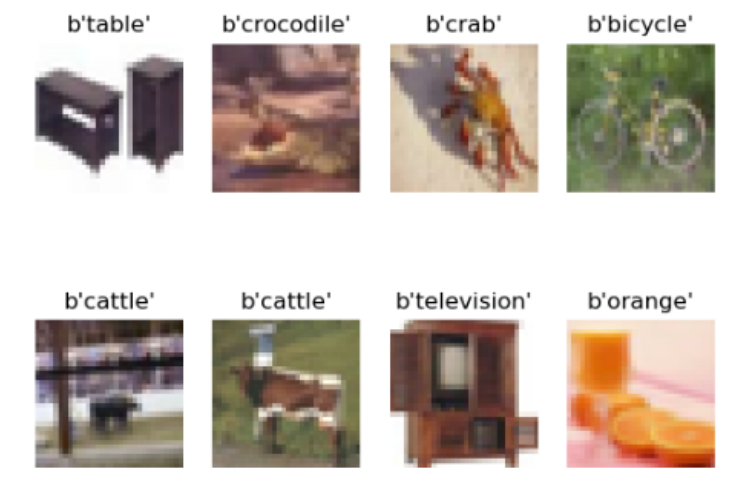
\includegraphics[width=\linewidth]{bench/img/cifar100.png}\\[3pt]
{\scriptsize CIFAR-100, 100 classes, 32$\times$32}
\end{center}
\end{minipage}

\begin{thebibliography}{10}
\beamertemplatearticlebibitems
\tiny
\bibitem{PruningBench} C. Li \emph{et al.}, A Comprehensive Study of Structural
Pruning for Vision Models (2025)
\end{thebibliography}

\end{frame}


% ------------------------------ SLIDE 7 ------------------------------
\begin{frame}
\frametitle{Latency of the pruned models}
\framesubtitle{Edge TPU speed-up versus parameter reduction, and INT8 model size}

\benchlegendfit{leg:benchspeedup}

\begin{center}
\makebox[\linewidth][c]{%
\begin{tikzpicture}
\begin{axis}[benchpanel, scale only axis, width=2.5cm, height=2.5cm, name=pVGG,
  title={VGG-19}, title style={font=\small, yshift=0.62cm},
  xlabel={Parameter reduction (\%)},
  ylabel={Edge TPU speed-up ($\times$)},
  xmin=0, xmax=90, xtick={0,30,60,90}, enlarge x limits=false]
\addplot[mark=none, domain=0:90, samples=2, dashed, black, thin] {1};
\benchseven{bench/data/sp_vgg19.csv}
\draw[red!70!black, dash dot, thick] ({axis cs:58.76,0}|-{rel axis cs:0,0}) -- ({axis cs:58.76,0}|-{rel axis cs:0,1});
\end{axis}
\begin{axis}[scale only axis, width=2.5cm, height=2.5cm,
  at=(pVGG.south west), anchor=south west,
  axis x line*=top, axis y line=none, ytick=\empty, ymin=0, ymax=1,
  xmin=1.93, xmax=19.30, x dir=reverse, enlarge x limits=false,
  xtick={2,6,10,14,18}, tick label style={font=\scriptsize},
  xlabel={INT8 size (MB)}, label style={font=\scriptsize}]
\end{axis}
\end{tikzpicture}\hspace{0.3cm}
\begin{tikzpicture}
\begin{axis}[benchpanel, scale only axis, width=2.5cm, height=2.5cm, name=pR18,
  title={ResNet-18}, title style={font=\small, yshift=0.62cm},
  xlabel={Parameter reduction (\%)},
  xmin=0, xmax=90, xtick={0,30,60,90}, enlarge x limits=false]
\addplot[mark=none, domain=0:90, samples=2, dashed, black, thin] {1};
\benchseven{bench/data/sp_resnet18.csv}
\draw[red!70!black, dash dot, thick] ({axis cs:26.29,0}|-{rel axis cs:0,0}) -- ({axis cs:26.29,0}|-{rel axis cs:0,1});
\end{axis}
\begin{axis}[scale only axis, width=2.5cm, height=2.5cm,
  at=(pR18.south west), anchor=south west,
  axis x line*=top, axis y line=none, ytick=\empty, ymin=0, ymax=1,
  xmin=1.08, xmax=10.84, x dir=reverse, enlarge x limits=false,
  xtick={2,4,6,8,10}, tick label style={font=\scriptsize},
  xlabel={INT8 size (MB)}, label style={font=\scriptsize}]
\end{axis}
\end{tikzpicture}\hspace{0.3cm}
\begin{tikzpicture}
\begin{axis}[benchpanel, scale only axis, width=2.5cm, height=2.5cm, name=pGLN,
  title={GoogLeNet}, title style={font=\small, yshift=0.62cm},
  xlabel={Parameter reduction (\%)},
  xmin=0, xmax=90, xtick={0,30,60,90}, enlarge x limits=false]
\addplot[mark=none, domain=0:90, samples=2, dashed, black, thin] {1};
\benchseven{bench/data/sp_googlenet.csv}
\end{axis}
\begin{axis}[scale only axis, width=2.5cm, height=2.5cm,
  at=(pGLN.south west), anchor=south west,
  axis x line*=top, axis y line=none, ytick=\empty, ymin=0, ymax=1,
  xmin=0.57, xmax=5.66, x dir=reverse, enlarge x limits=false,
  xtick={1,2,3,4,5}, tick label style={font=\scriptsize},
  xlabel={INT8 size (MB)}, label style={font=\scriptsize}]
\end{axis}
\end{tikzpicture}}

\vspace{3pt}
\ref{leg:benchspeedup}

\vspace{3pt}
{\small Red line: the rate at which the model first fits entirely on chip.
Note that each panel has its own vertical scale.}
\end{center}

\end{frame}


% ------------------------------ SLIDE 8 ------------------------------
\begin{frame}
\frametitle{Accuracy}
\framesubtitle{ResNet-18: accuracy right after pruning, and recovery fine-tuning}

\benchlegend{leg:benchacc}

\begin{center}
\makebox[\linewidth][c]{%
\begin{tikzpicture}
\begin{groupplot}[
  group style={group size=2 by 1, horizontal sep=1.5cm},
  benchpanel, scale only axis, width=3.1cm, height=3.1cm,
  title style={font=\small}]

\nextgroupplot[title={After pruning, before FT},
               xlabel={Pruning target (\%)}, ylabel={Top-1 val.\ acc.\ (\%)},
               xtick={10,30,50,70,90}]
\addplot[mark=none, domain=10:90, samples=2, dashed, black, thin] {76.890};
\benchseven{bench/data/pp_resnet18.csv}

\nextgroupplot[title={Recovery FT at 90\,\%},
               xlabel={Epoch}, ylabel={Top-1 val.\ acc.\ (\%)},
               xtick={0,50,100}]
\addplot[mark=none, domain=0:100, samples=2, dashed, black, thin, forget plot] {76.890};
\addplot[benchcurves, color=impmagnitudel1] table[x=epoch, y=magnitude_l1, col sep=comma] {bench/data/ft_resnet18_90.csv};
\addplot[benchcurves, color=impmagnitudel2] table[x=epoch, y=magnitude_l2, col sep=comma] {bench/data/ft_resnet18_90.csv};
\addplot[benchcurves, color=impbnscale]     table[x=epoch, y=bn_scale,     col sep=comma] {bench/data/ft_resnet18_90.csv};
\addplot[benchcurves, color=impfpgm]        table[x=epoch, y=fpgm,         col sep=comma] {bench/data/ft_resnet18_90.csv};
\addplot[benchcurves, color=imptaylor]      table[x=epoch, y=taylor,       col sep=comma] {bench/data/ft_resnet18_90.csv};
\addplot[benchcurves, color=impobdc]        table[x=epoch, y=obdc,         col sep=comma] {bench/data/ft_resnet18_90.csv};
\addplot[benchcurves, color=imprandom]      table[x=epoch, y=random,       col sep=comma] {bench/data/ft_resnet18_90.csv};

\end{groupplot}
\end{tikzpicture}}

\vspace{3pt}
\ref{leg:benchacc}

\vspace{3pt}
{\small Dashed line: unpruned baseline. Both indicators give the same ranking.}
\end{center}

\end{frame}


% ------------------------------ SLIDE 9 -----------------------------
\begin{frame}
\frametitle{Accuracy and latency disagree}
\framesubtitle{ResNet-50: the criterion that best preserves accuracy is the slowest}

\benchlegendfit{leg:benchboth}

\begin{center}
\makebox[\linewidth][c]{%
\begin{tikzpicture}
\begin{groupplot}[
  group style={group size=2 by 1, horizontal sep=1.5cm},
  benchpanel, scale only axis, width=3.1cm, height=3.1cm,
  title style={font=\small},
  xlabel={Parameter reduction (\%)}]

\nextgroupplot[title={Accuracy right after pruning},
               ylabel={Top-1 val.\ acc.\ (\%)}]
\addplot[mark=none, domain=10:90, samples=2, dashed, black, thin] {77.810};
\benchseven{bench/data/pp_resnet50.csv}

\nextgroupplot[title={Edge TPU speed-up}, ylabel={Speed-up ($\times$)}]
\addplot[mark=none, domain=0:90, samples=2, dashed, black, thin] {1};
\benchseven{bench/data/sp_resnet50.csv}
\draw[red!70!black, dash dot, thick] ({axis cs:65.90,0}|-{rel axis cs:0,0}) -- ({axis cs:65.90,0}|-{rel axis cs:0,1});

\end{groupplot}
\end{tikzpicture}}

\vspace{2pt}
\ref{leg:benchboth}

\vspace{2pt}
{\small At equal parameter reduction, two criteria do not produce the same
on-chip footprint: \emph{where} channels are removed matters.}
\end{center}

\end{frame}


% ------------------------------ SLIDE 10 -----------------------------
\begin{frame}
\frametitle{Real-time scheduling of multiple DNNs on a single TPU}
\framesubtitle{Illustrative use case}

\begin{minipage}{0.64\textwidth}
{\small
\begin{itemize}\setlength{\itemsep}{3pt}
  \item[{\color{blue!80!black}$\bullet$}] Single TPU
  \item[{\color{blue!80!black}$\bullet$}] Many DNNs executed at different rates
  \item[{\color{blue!80!black}$\bullet$}] \emph{Earliest Deadline First (EDF)}
  \item[{\color{blue!80!black}$\bullet$}] Non-preemptive avoids weight reloading
  \item[{\color{blue!80!black}$\bullet$}] Sporadic tasks (\emph{i.e.,} event-triggered)
\end{itemize}}

\vspace{0.25cm}

\setlength{\tabcolsep}{4pt}
\renewcommand{\arraystretch}{0.95}
{\tiny
\begin{tabular}{llrrr}
\toprule
Function & Model & $T$ (ms) & $C$ (ms) & $C/T$ \\
\midrule
Nozzle trigger    & ResNet-18    &  20 & 11.4 & 0.57 \\
Crop growth stage & MobileNetV2  &  33 &  1.2 & 0.04 \\
Weed species      & ResNet-50    & 100 & 50.9 & 0.51 \\
Ground cover      & VGG-19       & 200 & 39.3 & 0.20 \\
\midrule
\multicolumn{4}{r}{Total utilization} & \textbf{\color{red!80!black}1.32} \\
\bottomrule
\end{tabular}}

\vspace{0.2cm}
{\small \color{red!80!black}$U > 1$ : the task set is \textbf{infeasible}.}
\end{minipage}\hfill
\begin{minipage}{0.32\textwidth}
\begin{center}
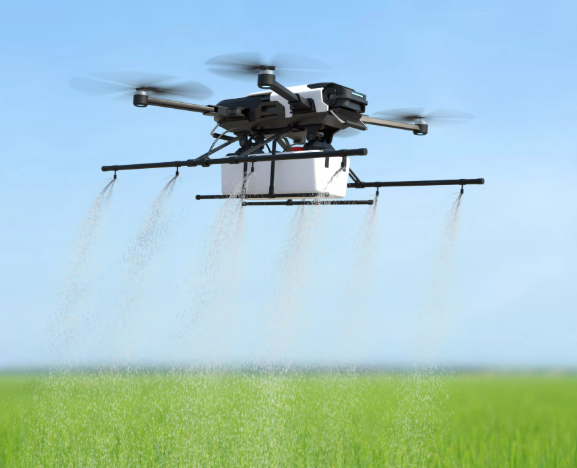
\includegraphics[width=\linewidth]{bench/img/drone_rampe_de_buses.png}\\[5pt]
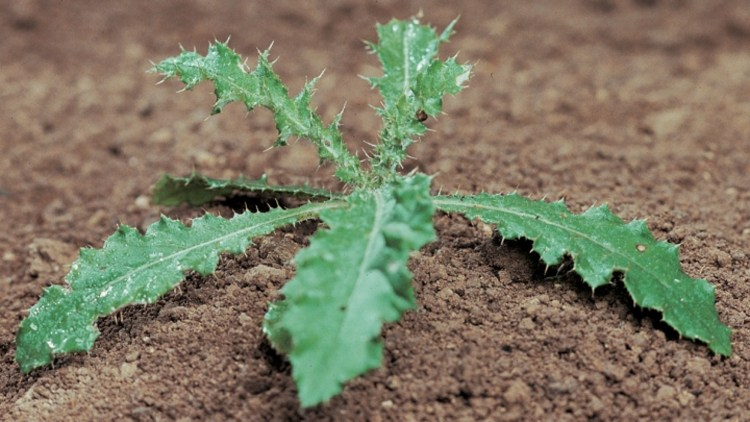
\includegraphics[width=\linewidth]{bench/img/adventice.jpg}
\end{center}
\end{minipage}

\vspace{0.2cm}

\begin{thebibliography}{10}
\beamertemplatearticlebibitems
\tiny
\bibitem{Buttazzo} G. Buttazzo, Can We Trust AI-Powered Real-Time Embedded
Systems? NG-RES (2022)
\end{thebibliography}

\end{frame}




\begin{frame}
\frametitle{Periodic task scheduling}

\begin{minipage}{0.25\textwidth} 	                        
\begin{center}
		{\small
			\begin{tabular}{l|cccc}
				& $C_i$     & $T_i$ & $A_i$ \\ \hline
				\only<1>{$\tau_1$ & $0.50$ & $2.00$ & $80.00\%$  \\
				$\tau_2$ & $0.50$ & $4.00$ & $75.00\%$\\
				$\tau_3$ & $0.50$ & $6.00$ & $90.00\%$}\only<2>{$\tau_1$ & $1.00$ & $2.00$ & $88.00\%$  \\
				$\tau_2$ & $1.00$ & $4.00$ & $82.00\%$\\
				$\tau_3$ & $1.00$ & $6.00$ & $93.00\%$}\only<3>{$\tau_1$ & $1.50$ & $2.00$ & $94.00\%$  \\
				$\tau_2$ & $1.50$ & $4.00$ & $88.00\%$\\
				$\tau_3$ & $1.00$ & $6.00$ & $93.00\%$}
			\end{tabular}
		}
	\end{center}
	\end{minipage}          
	\begin{minipage}{0.15\textwidth}              
	$ $             
	\end{minipage}
	\begin{minipage}{0.55\textwidth}        
		{       \small
			Each sporadic task $\tau_i$ is characterized by:\\
			\hspace*{0.2cm} \mbox{$C_i$ worst-case inference time}\\
			\hspace*{0.2cm} $T_i$ minimum inter-arrival time (\emph{period}) \\
			\hspace*{0.2cm} $A_i$ accuracy
		}
\end{minipage}

\vspace*{0.5cm}


	
\begin{RTGrid}[width=.9\textwidth, height=4cm, nogrid=1, nonumbers=1,nosymbols=1]{3}{7}
	\TaskNArrival{1}{0}{2.0}{4}
	\TaskNArrival{2}{0}{4.0}{2}
	\TaskNArrival{3}{0}{6.0}{2}
	
\only<1>{	
	\TaskExecution[color=red!50]{1}{0}{0.5}
	\TaskExecution[color=red!50]{1}{2}{2.5}
	\TaskExecution[color=red!50]{1}{4}{4.5}
	\TaskExecution[color=red!50]{1}{6}{6.5}
	\TaskExecution[color=blue!50]{2}{0.5}{1.0}
	\TaskExecution[color=blue!50]{2}{4.5}{5.0}
	\TaskExecution[color=green!50]{3}{1.0}{1.5}
}
\only<2>{	
	\TaskExecution[color=red!50]{1}{0}{1}
	\TaskExecution[color=red!50]{1}{2}{3}
	\TaskExecution[color=red!50]{1}{4}{5}
	\TaskExecution[color=red!50]{1}{6}{6.7}
	\TaskExecution[color=blue!50]{2}{1}{2}
	\TaskExecution[color=blue!50]{2}{5}{6}
	\TaskExecution[color=green!50]{3}{3}{4}
}
\only<3>{	
	\TaskExecution[color=red!50]{1}{0}{1.5}
	\TaskExecution[color=red!50]{1}{3.0}{4.0}
	\TaskExecution[color=red!90!black]{1}{4.0}{4.5}
	\TaskExecution[color=red!50]{1}{4.5}{6}
	\TaskExecution[color=red!50]{1}{6}{6.7}
	\TaskExecution[color=blue!50]{2}{1.5}{3.0}
	%\TaskExecution[color=blue!50]{2}{5}{6}
	%\TaskExecution[color=green!50]{3}{3.5}{4.5}
}


	\node at (0.8,3.2) {$\tau_1$};
	\node at (0.8,2.0) {$\tau_2$};
	\node at (0.8,0.8) {$\tau_3$};

	\node at (1.1,0.15) {\footnotesize $0$};
	%\node at (1.80,0.15) {\footnotesize $1$};
	\node at (7.55,0.15) {\footnotesize $6$};
	
	\node at (1.1,1.4) {\footnotesize $0$};
	%\node at (3.55,1.4) {\footnotesize $3$};
	\node at (5.4,1.4) {\footnotesize $4$};
	
	
	\node at (1.1,2.55) {\footnotesize $0$};
	%\node at (1.80,2.55) {\footnotesize $1$};
	\node at (3.2,2.55) {\footnotesize $2$};
	\node at (5.4,2.55) {\footnotesize $4$};
	\node at (7.55,2.55) {\footnotesize $6$};
    
   % \draw[decorate,decoration={brace,amplitude=5pt}] (3.55,-0.15) -- (0.9,-0.15) node[pos=0.5, yshift=-0.5cm] {\small $s_2{=}3$};
%	\draw[dotted] (3.55,1.5) -- (3.55,-0.15);

	\node at (2.0,-0.9) {};
	
	
	\only<1>{
	\node[text width=3cm,align=center] at (10.5,1.6) {Schedulable but low accuracy};
	}
	
	\only<2>{
		\node[text width=3cm,align=center] at (10.5,1.6) {Schedulable and good accuracy};
	}
	
	\only<3>{
		\node[text width=3cm,align=center] at (10.5,1.6) {High accuracy but not schedulable};
	}
	%\draw[decorate,decoration={brace,amplitude=5pt}] (4.4,-0.9) -- (0.9,-0.9) node[pos=0.5, yshift=-0.5cm] {\small $R_2{=}4$};

	%\draw[dotted] (4.4,1.5) -- (4.4,-0.9);

\end{RTGrid}

\end{frame}


\begin{frame}
\frametitle{Non-preemptive EDF schedulability test}


\vspace*{-0.1cm}


\begin{minipage}{0.20\textwidth} 	                        
	\begin{center}
		{\small
			\begin{tabular}{l|cccc}
				& $C_i$     & $T_i$  \\ \hline
				$\tau_1$ & $1.00$ & $2.00$   \\
					$\tau_2$ & $1.00$ & $4.00$ \\
					$\tau_3$ & $0.50$ & $6.00$ 
			\end{tabular}
		}
	\end{center}
\end{minipage}          
\begin{minipage}{0.1\textwidth}              
	$ $             
\end{minipage}
\begin{minipage}{0.65\textwidth}        
	{       \small
		 Sort tasks in non-decreasing order of  periods.
		
		For $k$ from $1$ to $n$:
		\vspace*{-0.3cm}
		\begin{equation*}
			\frac{B_k}{T_k} + \sum_{i=1}^k \frac{C_i}{T_i} \leq 1
		\end{equation*}
		\hspace*{1.3cm}	where $B_k = \max \{ C_j \, | \, T_j > T_k\}$  
	}
\end{minipage}
	


\begin{RTGrid}[width=.9\textwidth, height=3.8cm, nogrid=1, nonumbers=1,nosymbols=1]{3}{7}
	\TaskNArrival{1}{0}{2.0}{4}
	\TaskNArrival{2}{0}{4.0}{2}
	\TaskNArrival{3}{0}{6.0}{2}

%\only<1>{		
%	\TaskExecution[color=red!50]{1}{1}{2}
%	\TaskExecution[color=red!50]{1}{2}{3}
%	\TaskExecution[color=red!50]{1}{4}{5}
%	\TaskExecution[color=red!50]{1}{6}{6.7}
%	\TaskExecution[color=blue!50]{2}{0}{1}
%	\TaskExecution[color=blue!50]{2}{5}{6}
%	\TaskExecution[color=green!50]{3}{3}{3.5}
%}

%\only<2>{		
	\TaskExecution[color=red!50]{1}{0.5}{1.5}
	\TaskExecution[color=red!50]{1}{2.5}{3.5}
	\TaskExecution[color=red!50]{1}{4}{5}
	\TaskExecution[color=red!50]{1}{6}{6.7}
	\TaskExecution[color=blue!50]{2}{1.5}{2.5}
	\TaskExecution[color=blue!50]{2}{5}{6}
	\TaskExecution[color=green!50]{3}{0}{0.5}
%}
	
%\only<3>{		
%		\TaskExecution[color=red!50]{1}{0}{1}
%		\TaskExecution[color=red!50]{1}{2.5}{3.5}
%		\TaskExecution[color=red!50]{1}{4}{5}
%		\TaskExecution[color=red!50]{1}{6}{6.7}
%		\TaskExecution[color=blue!50]{2}{1}{2.5}
%		\TaskExecution[color=blue!50]{2}{5}{6}
%		\TaskExecution[color=green!50]{3}{3.5}{4}
%}
	
	\node at (0.8,3.2) {$\tau_1$};
	\node at (0.8,2.0) {$\tau_2$};
	\node at (0.8,0.8) {$\tau_3$};
	
	\node at (1.1,0.2) {\footnotesize $0$};
	%\node at (1.80,0.15) {\footnotesize $1$};
	\node at (7.55,0.2) {\footnotesize $6$};
	
	\node at (1.1,1.3) {\footnotesize $0$};
	%\node at (3.55,1.4) {\footnotesize $3$};
	\node at (5.4,1.3) {\footnotesize $4$};
	
	
	\node at (1.1,2.45) {\footnotesize $0$};
	%\node at (1.80,2.55) {\footnotesize $1$};
	\node at (3.2,2.45) {\footnotesize $2$};
	\node at (5.4,2.45) {\footnotesize $4$};
	\node at (7.55,2.45) {\footnotesize $6$};
	
	% \draw[decorate,decoration={brace,amplitude=5pt}] (3.55,-0.15) -- (0.9,-0.15) node[pos=0.5, yshift=-0.5cm] {\small $s_2{=}3$};
	%	\draw[dotted] (3.55,1.5) -- (3.55,-0.15);
	
	\node at (2.0,-0.9) {};
	

	\draw[decorate,decoration={brace,amplitude=5pt}] (5.4,-0.0) -- (1.2,-0.0) node[pos=0.5, yshift=-0.3cm] {\scriptsize $T_2{=}4$};
	
	\draw[dotted] (5.4,3.0) -- (5.4,0.0);
\end{RTGrid}


\vspace*{-1.2cm}

{\small 
\begin{equation*}
\text{For } k{=}2:	B_2/T_2 + C_1/T_1 + C_2/T_2 = 0.5/4+1/2+1/4 =  0.875 \leq 1
\end{equation*}
}



\begin{thebibliography}{10}
	\beamertemplatearticlebibitems
	
	\tiny
	\bibitem{Jeffay} K. Jeffay, D.F. Stanat and C.U. Martel, On non-preemptive
	scheduling of period and sporadic tasks (1991)
\end{thebibliography}


\end{frame}




\begin{frame}
	\frametitle{0–1 Integer Linear Programming  (ILP)  model}

{\scriptsize 	 
\begin{align}
	\text{max.}~
	& \sum_{i=1}^n \sum_{j=1}^m
	\frac{A_i^j}{T_i} \cdot x_i^j &&
	&& \text{\color{blue!60!black}Maximize accuracy}
	\label{model:obj}\\
	\text{s.t.}~
	& B_k/T_k + \sum_{i=1}^k \sum_{j=1}^m
	x_i^j \cdot C_i^j/T_i \leq 1,
	&& \forall\, 1 \leq k \leq n
	&& \text{\color{blue!60!black}Schedulability test}
	\label{model:const_sched}\\
	& B_k \geq C_i^j \cdot x_i^j,
	&& \forall\, k < i \leq n,
	&& \text{\color{blue!60!black}Blocking factor} 
	 \\
	& 
	&& \forall\, 1 \leq j \leq m
	&& \nonumber  \\
	& \sum_{j=1}^m x_i^j = 1,
	&& \forall\, 1 \leq i \leq n
	&& \text{\color{blue!60!black}One assignment}
	\label{model:const_only_one}\\
	& x_i^j \in \{0,1\},
	&& \forall\, 1 \leq i \leq n,
	&& \text{\color{blue!60!black}Binary decision} 
	\label{model:const_binary} \nonumber\\
	&  
	&& 
	1 \leq j \leq m
	&& \text{\color{blue!60!black}variables}
\end{align}


}
\end{frame}


\begin{frame}
\frametitle{Branch-and-bound  (B\&B)}
	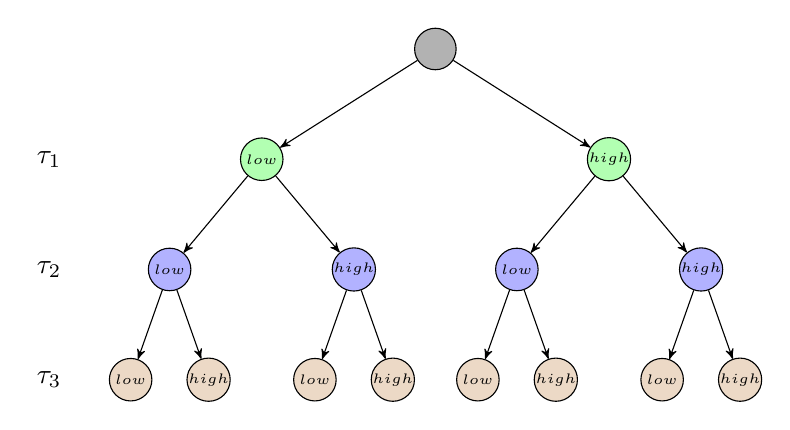
\begin{tikzpicture}[xscale=0.45,->,>=stealth',
		level 1/.style={sibling distance=9.8cm, level distance=1.4cm},
		level 2/.style={sibling distance=5.2cm, level distance=1.4cm},
		level 3/.style={sibling distance=2.2cm, level distance=1.4cm}]
		
		\tikzset{
			treenode/.style = {align=center, inner sep=0pt, text centered,
				font=\sffamily},
			node_1/.style = {treenode, circle, draw=black, fill=green!30,
				text width=1.5em, minimum size=1.5em,font=\tiny},
			node_n/.style = {treenode, circle, draw=black, fill=blue!30,
				text width=1.5em, minimum size=1.5em,font=\tiny},
			node_0/.style = {treenode, circle, draw=black, fill=black!30,
				text width=1.5em, minimum size=1.5em,font=\tiny},
			node_3/.style = {treenode, circle, draw=black, fill=brown!30,
				text width=1.5em, minimum size=1.5em,font=\tiny}
		}
		% Root node
		\node [node_0] (root) {}
		child{ node [node_1] (A) {\tiny $low$}
			child{ node [node_n] (A2) {$low$}
				child{ node [node_3] (A3) {$low$} edge from parent node[pos=0.7] {}}
				child{ node [node_3] (t32) {$high$} edge from parent node[pos=0.7]  {}}
				edge from parent node[xshift=-0.1cm,pos=0.7] {}
			}
			child{ node [node_n] {$high$}
				child{ node  [node_3] (t33) {$low$} edge from parent node[pos=0.7] {}}
				child{ node [node_3] (t34) {$high$} edge from parent node[pos=0.7] {}}
				edge from parent node[xshift=-0.1cm,pos=0.7] {}
			}
		}
		child{ node [node_1] (B) {$high$}
			child{ node [node_n] {$low$}
				child{ node [node_3] (t35) {$low$} edge from parent node[pos=0.7] {}}
				child{ node [node_3] (t36) {$high$} edge from parent node[pos=0.5,xshift=0.5cm] {}}
				edge from parent node[xshift=-0.6cm,pos=0.5] {}
			}
			child{ node [node_n] {$high$}
				child{ node [node_3] (t37) {$low$} edge from parent node[pos=0.5,xshift=-0.45cm] {}}
				child{ node [node_3] (t38) {$high$} edge from parent node[pos=0.5] {  }}
				edge from parent node[xshift=0.6cm,pos=0.5] {}
			}
		};
		
		\path (root) -- (A) node[midway, above, xshift=-0.3cm] {};
		\path (root) -- (B) node[midway, above, xshift=0.3cm] { };
		
		\node at ($(A)+(-6cm,0)$) (t1) {$\tau_1$};
		\node at (A2 -| t1) {$\tau_2$};
		\node at (A3 -| t1) {$\tau_3$};
		
		
		\end{tikzpicture}
		
		\begin{block}{}
			Each level represents a task ($\tau_1, \tau_2, \tau_3$).\\
			Each node  represents an accuracy (\emph{low} or \emph{high}).\\
			{\scriptsize low accuracy $\implies$ low inference times while  high accuracy $\implies$ high inference times.}
			Find a pruning rate assignment for each task such that:\\ 
			i) the average precision is maximized, and ii) tasks are schedulable.
		\end{block}
		
		
		
\end{frame}


\begin{frame}
	\frametitle{Branch-and-bound  (B\&B)}
	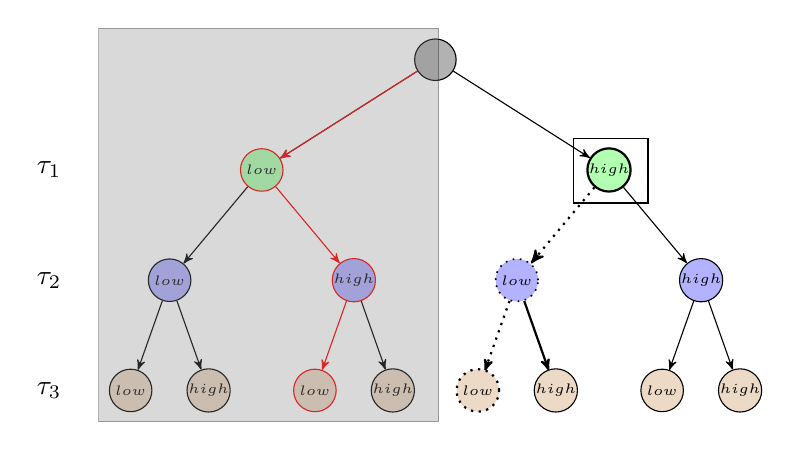
\begin{tikzpicture}[xscale=0.45,->,>=stealth',
		level 1/.style={sibling distance=9.8cm, level distance=1.4cm},
		level 2/.style={sibling distance=5.2cm, level distance=1.4cm},
		level 3/.style={sibling distance=2.2cm, level distance=1.4cm}]
		
		\tikzset{
			treenode/.style = {align=center, inner sep=0pt, text centered,
				font=\sffamily},
			node_1/.style = {treenode, circle, draw=black, fill=green!30,
				text width=1.5em, minimum size=1.5em,font=\tiny},
			node_n/.style = {treenode, circle, draw=black, fill=blue!30,
				text width=1.5em, minimum size=1.5em,font=\tiny},
			node_0/.style = {treenode, circle, draw=black, fill=black!30,
				text width=1.5em, minimum size=1.5em,font=\tiny},
			node_3/.style = {treenode, circle, draw=black, fill=brown!30,
				text width=1.5em, minimum size=1.5em,font=\tiny}
		}
		% Root node
		\node [node_0] (root) {}
		child{ node [node_1,draw=red] (A) {\tiny $low$}
			child{ node [node_n] (A2) {$low$}
				child{ node [node_3] (A3) {$low$} edge from parent node[pos=0.7] {}}
				child{ node [node_3] (t32) {$high$} edge from parent node[pos=0.7]  {}}
				edge from parent node[xshift=-0.1cm,pos=0.7] {}
			}
			child{ node [node_n,draw=red] {$high$}
				child{ node  [node_3,draw=red] (t33) {$low$} edge from parent node[pos=0.7] {}}
				child{ node [node_3] (t34) {$high$} edge from parent[black] node[pos=0.7] {}}
				edge from parent[red] node[xshift=-0.1cm,pos=0.7] {}
			}
		}
		child{ node [node_1,thick] (B) {$high$}
			child{ node [node_n,dotted,semithick] {$low$}
				child{ node [node_3] (t35) {$low$} edge from parent node[pos=0.7] {}}
				child{ node [node_3,thin,solid] (t36) {$high$} edge from parent[solid] node[pos=0.5,xshift=0.5cm] {}}
				edge from parent[dotted,thick] node[xshift=-0.6cm,pos=0.5,solid] {}
			}
			child{ node [node_n] {$high$}
				child{ node [node_3] (t37) {$low$} edge from parent node[pos=0.5,xshift=-0.45cm] {}}
				child{ node [node_3] (t38) {$high$} edge from parent node[pos=0.5] {}}
				edge from parent node[xshift=0.6cm,pos=0.5] {}
			}
		};
		
		\path[draw=red] (root) -- (A) node[midway, above, xshift=-0.3cm] {};
		\path (root) -- (B) node[midway, above, xshift=0.3cm] { };
		
		\node at ($(A)+(-6cm,0)$) (t1) {$\tau_1$};
		\node at (A2 -| t1) {$\tau_2$};
		\node at (A3 -| t1) {$\tau_3$};
		
		\draw (3.9,-1) rectangle (6,-1.82);
		\draw[opacity=0.3,fill=gray] (-9.5,0.4) rectangle (0.1,-4.6);
		
	\end{tikzpicture}
	
	
	\begin{block}{Current state}
		Left sub-tree has been explored, we are at $\tau_1\gets high$, and\\ 
		$\tau_1 \gets low, \tau_2\gets high, \tau_3 \gets low$ is the best solution found so far.
	\end{block}
	
	\begin{block}{Schedulability branch-pruning}
	If $\tau_1 \gets high, \tau_2\gets \textbf{low}, \tau_3 \gets \textbf{low}$ is not schedulable then no other assignment can be schedulable.
	\end{block}
	
\end{frame}


\begin{frame}
	\frametitle{Branch-and-bound  (B\&B)}
	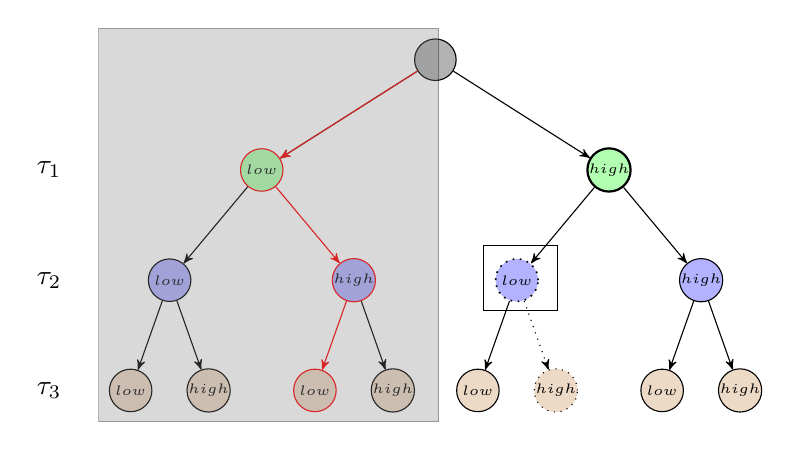
\begin{tikzpicture}[xscale=0.45,->,>=stealth',
		level 1/.style={sibling distance=9.8cm, level distance=1.4cm},
		level 2/.style={sibling distance=5.2cm, level distance=1.4cm},
		level 3/.style={sibling distance=2.2cm, level distance=1.4cm}]
		
		\tikzset{
			treenode/.style = {align=center, inner sep=0pt, text centered,
				font=\sffamily},
			node_1/.style = {treenode, circle, draw=black, fill=green!30,
				text width=1.5em, minimum size=1.5em,font=\tiny},
			node_n/.style = {treenode, circle, draw=black, fill=blue!30,
				text width=1.5em, minimum size=1.5em,font=\tiny},
			node_0/.style = {treenode, circle, draw=black, fill=black!30,
				text width=1.5em, minimum size=1.5em,font=\tiny},
			node_3/.style = {treenode, circle, draw=black, fill=brown!30,
				text width=1.5em, minimum size=1.5em,font=\tiny}
		}
		% Root node
		\node [node_0] (root) {}
		child{ node [node_1,draw=red] (A) {\tiny $low$}
			child{ node [node_n] (A2) {$low$}
				child{ node [node_3] (A3) {$low$} edge from parent node[pos=0.7] {}}
				child{ node [node_3] (t32) {$high$} edge from parent node[pos=0.7]  {}}
				edge from parent node[xshift=-0.1cm,pos=0.7] {}
			}
			child{ node [node_n,draw=red] {$high$}
				child{ node  [node_3,draw=red] (t33) {$low$} edge from parent node[pos=0.7] {}}
				child{ node [node_3] (t34) {$high$} edge from parent[black] node[pos=0.7] {}}
				edge from parent[red] node[xshift=-0.1cm,pos=0.7] {}
			}
		}
		child{ node [node_1,thick] (B) {$high$}
			child{ node [node_n,dotted,semithick] {$low$}
				child{ node [node_3] (t35) {$low$} edge from parent node[pos=0.7] {}}
				child{ node [node_3,dotted] (t36) {$high$} edge from parent[dotted] node[pos=0.5,xshift=0.5cm] {}}
				edge from parent node[xshift=-0.6cm,pos=0.5,solid] {}
			}
			child{ node [node_n] {$high$}
				child{ node [node_3] (t37) {$low$} edge from parent node[pos=0.5,xshift=-0.45cm] {}}
				child{ node [node_3] (t38) {$high$} edge from parent node[pos=0.5] {}}
				edge from parent node[xshift=0.6cm,pos=0.5] {}
			}
		};
		
		\path[draw=red] (root) -- (A) node[midway, above, xshift=-0.3cm] {};
		\path (root) -- (B) node[midway, above, xshift=0.3cm] { };
		
		\node at ($(A)+(-6cm,0)$) (t1) {$\tau_1$};
		\node at (A2 -| t1) {$\tau_2$};
		\node at (A3 -| t1) {$\tau_3$};
		
		\draw (1.9-0.55,-1-1.36) rectangle (4-0.55,-1.82-1.36);
		\draw[opacity=0.3,fill=gray] (-9.5,0.4) rectangle (0.1,-4.6);
		
	\end{tikzpicture}
	
	
	\begin{block}{Current state}
		Left sub-tree has been explored, we are at $\tau_1\gets high, \tau_2\gets low$, and\\ 
		\mbox{$\tau_1 \gets low, \tau_2\gets high, \tau_3 \gets low$ is still the best solution found so~far.}
	\end{block}
	
	\begin{block}{Accuracy branch-pruning}
		If $\tau_1 \gets high, \tau_2\gets low, \tau_3 \gets \textbf{high}$ does not have better accuracy then no other assignment can be better (\emph{i.e.,} $\tau_3 \gets low$).
	\end{block}
	
\end{frame}

\begin{frame}
	\frametitle{Schedulability experiments}
	\framesubtitle{Schedulability ratio with and without pruning}

\begin{minipage}[c]{0.35\textwidth}
{\scriptsize\raggedright
\begin{itemize}\setlength{\itemsep}{7pt}\setlength{\leftmargini}{1.1em}
  \setlength{\rightmargin}{0pt}
  \item[{\color{blue!80!black}$\bullet$}]
    Random task sets of \textbf{six tasks}, utilizations drawn with
    \textbf{RandFixedSum}.
  \item[{\color{blue!80!black}$\bullet$}]
    \textbf{250 task sets} per utilization point, from $0.1$ to $4.0$.
  \item[{\color{blue!80!black}$\bullet$}]
    Periods sampled \textbf{log-uniformly} between $10$ and $100$\,ms.
  \item[{\color{blue!80!black}$\bullet$}]
    Each task takes its \textbf{profile at random} from the benchmark.
\end{itemize}}
\end{minipage}\hfill
\begin{minipage}[c]{0.61\textwidth}
	\begin{center}
		
		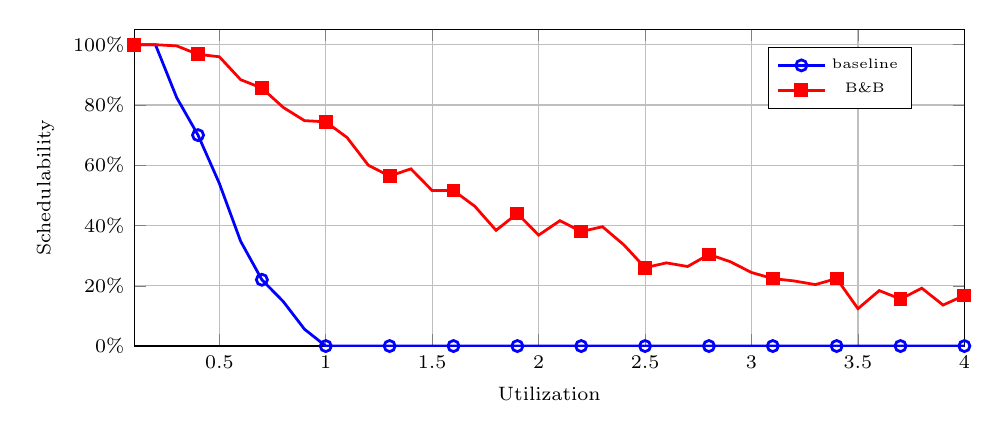
\begin{tikzpicture}
			\begin{axis}[
				width=\linewidth,
				height=5.6cm,
				xlabel={Utilization},
				ylabel={Schedulability},
				xmin=0.1, xmax=4.0,
				ymin=0, ymax=1.05,
				grid=both,
				tick label style={font=\scriptsize},
				label style={font=\scriptsize},
				ytick={0,0.2,0.4,0.6,0.8,1.0},
				yticklabel={\pgfmathparse{\tick*100}\pgfmathprintnumber{\pgfmathresult}\%},
				legend style={
					at={(0.85,0.75)},
					anchor=south,
					legend columns=1,
					font=\tiny,
				},
				mark size=2pt,
				]
				
				\addplot[
				blue,
				mark=o,
				mark repeat=3,
				line width=1pt
				] coordinates {
					(0.10,1.000)
					(0.20,1.000)
					(0.30,0.824)
					(0.40,0.700)
					(0.50,0.540)
					(0.60,0.348)
					(0.70,0.220)
					(0.80,0.148)
					(0.90,0.056)
					(1.00,0.000)
					(1.10,0.000)
					(1.20,0.000)
					(1.30,0.000)
					(1.40,0.000)
					(1.50,0.000)
					(1.60,0.000)
					(1.70,0.000)
					(1.80,0.000)
					(1.90,0.000)
					(2.00,0.000)
					(2.10,0.000)
					(2.20,0.000)
					(2.30,0.000)
					(2.40,0.000)
					(2.50,0.000)
					(2.60,0.000)
					(2.70,0.000)
					(2.80,0.000)
					(2.90,0.000)
					(3.00,0.000)
					(3.10,0.000)
					(3.20,0.000)
					(3.30,0.000)
					(3.40,0.000)
					(3.50,0.000)
					(3.60,0.000)
					(3.70,0.000)
					(3.80,0.000)
					(3.90,0.000)
					(4.00,0.000)
				};
				\addlegendentry{baseline}
				
				\addplot[
				red,
				mark=square*,
				mark repeat=3,
				line width=1pt
				] coordinates {
					(0.10,1.000)
					(0.20,1.000)
					(0.30,0.996)
					(0.40,0.968)
					(0.50,0.960)
					(0.60,0.884)
					(0.70,0.856)
					(0.80,0.792)
					(0.90,0.748)
					(1.00,0.744)
					(1.10,0.692)
					(1.20,0.600)
					(1.30,0.564)
					(1.40,0.588)
					(1.50,0.516)
					(1.60,0.516)
					(1.70,0.464)
					(1.80,0.384)
					(1.90,0.440)
					(2.00,0.368)
					(2.10,0.416)
					(2.20,0.380)
					(2.30,0.396)
					(2.40,0.336)
					(2.50,0.260)
					(2.60,0.276)
					(2.70,0.264)
					(2.80,0.304)
					(2.90,0.280)
					(3.00,0.244)
					(3.10,0.224)
					(3.20,0.216)
					(3.30,0.204)
					(3.40,0.224)
					(3.50,0.124)
					(3.60,0.184)
					(3.70,0.156)
					(3.80,0.192)
					(3.90,0.136)
					(4.00,0.168)
				};
				\addlegendentry{B\&B}
				
				
			\end{axis}
		\end{tikzpicture}
	
	\end{center}
\end{minipage}
	
\end{frame}


\begin{frame}
	\frametitle{Schedulability experiments}
	\framesubtitle{Accuracy drop with pruning for B\&B method}


\begin{center}
	
	   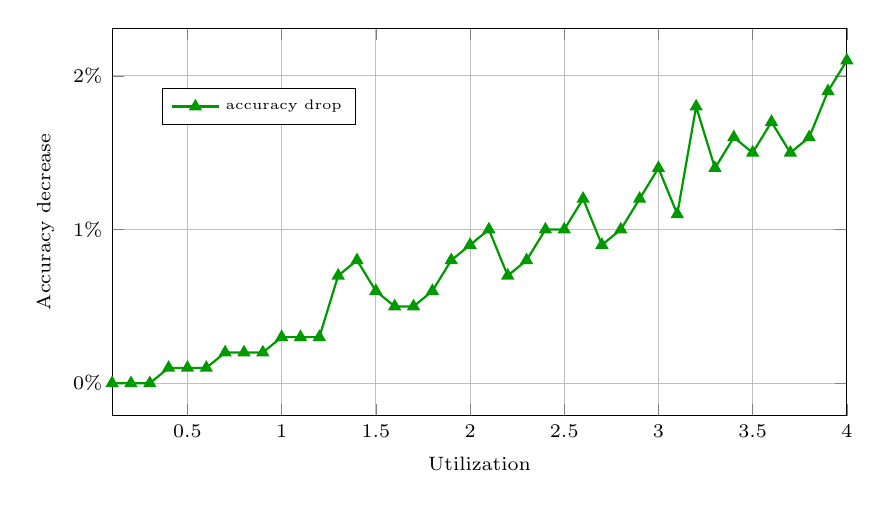
\begin{tikzpicture}
		\begin{axis}[
			width=0.9\linewidth,
			height=6.5cm,
			xlabel={Utilization},
			ylabel={Accuracy decrease},
			xmin=0.1, xmax=4.0,
			%ymin=0, ymax=0.05,
			grid=both,
			tick label style={font=\scriptsize},
			label style={font=\scriptsize},
			%ytick={0,0.005,0.010,0.015,0.020},
			yticklabel={\pgfmathparse{\tick}\pgfmathprintnumber{\pgfmathresult}\%},
			legend style={
				at={(0.20,0.75)},
				anchor=south,
				legend columns=1,
				font=\tiny,
			},
			mark size=2pt,
			]
			
			\addplot[
			green!60!black,
			mark=triangle*,
			thick
			] coordinates {
				(0.10,0.000)
				(0.20,0.000)
				(0.30,0.000)
				(0.40,0.1)
				(0.50,0.1)
				(0.60,0.1)
				(0.70,0.2)
				(0.80,0.2)
				(0.90,0.2)
				(1.00,0.3)
				(1.10,0.3)
				(1.20,0.3)
				(1.30,0.7)
				(1.40,0.8)
				(1.50,0.6)
				(1.60,0.5)
				(1.70,0.5)
				(1.80,0.6)
				(1.90,0.8)
				(2.00,0.9)
				(2.10,1.0)
				(2.20,0.7)
				(2.30,0.8)
				(2.40,1.0)
				(2.50,1.0)
				(2.60,1.2)
				(2.70,0.9)
				(2.80,1.0)
				(2.90,1.2)
				(3.00,1.4)
				(3.10,1.1)
				(3.20,1.8)
				(3.30,1.4)
				(3.40,1.6)
				(3.50,1.5)
				(3.60,1.7)
				(3.70,1.5)
				(3.80,1.6)
				(3.90,1.9)
				(4.00,2.1)
			};
			\addlegendentry{accuracy drop}
			
		\end{axis}
	\end{tikzpicture}

\end{center}	
	
\end{frame}


% =====================================================================
%  Frame de conclusion : formulations courtes, chiffres a l'appui.
% =====================================================================
\begin{frame}
\frametitle{Conclusion}

\begin{itemize}\setlength{\itemsep}{8pt}
  \item[{\color{blue!80!black}$\bullet$}]
    \textbf{Latency is a step function of model size.}\\
    {\small Up to $60\times$ below the 8\,MB threshold, at most $2\times$ above it.
     The knee is the on-chip capacity, not the parameter count.}
  \item[{\color{blue!80!black}$\bullet$}]
    \textbf{No importance criterion dominates both dimensions.}\\
    {\small Criterion selection is itself an accuracy--latency trade-off.}
  \item[{\color{blue!80!black}$\bullet$}]
    \textbf{Pruning rates are a scheduling variable.}\\
    {\small Schedulable well beyond the point where the unpruned system fails,
     for about 2\,\% of accuracy on the most loaded task sets.}
\end{itemize}

\vspace{0.9cm}
\begin{center}
{\color{blue!80!black}\textbf{Thank you for your attention.}}
\end{center}

\end{frame}


\end{document}
